\documentclass[aspectratio=169,10pt]{beamer}
\usetheme[progressbar=frametitle,numbering=fraction,sectionpage=none,block=fill]{metropolis}

% ---------------------------------------------------------------------------------------------
% Packages
% ---------------------------------------------------------------------------------------------
\usepackage[T1]{fontenc}
\usepackage[utf8]{inputenc}
\usepackage{lmodern}
\usepackage{amsmath,amssymb,bm}
\usepackage{booktabs,array,multirow}
\usepackage{listings}
\usepackage{tikz}
\usetikzlibrary{arrows.meta,calc,positioning,decorations.pathreplacing,patterns,fit,backgrounds}
\usepackage{pgfplots}
\usepgfplotslibrary{groupplots}
\pgfplotsset{compat=1.18}

% ---------------------------------------------------------------------------------------------
% Colours (same as the report): Schwarz blue, GAMG orange
% ---------------------------------------------------------------------------------------------
\definecolor{schwarz}{HTML}{2A6FDB}
\definecolor{gamg}{HTML}{E8642C}
\definecolor{accent}{HTML}{E8642C}
\definecolor{boxfill}{HTML}{F2F5FA}
\definecolor{boxedge}{HTML}{55657A}
\definecolor{codebg}{HTML}{F3F4F6}
\definecolor{ink2}{HTML}{52514E}
\definecolor{titlebg}{HTML}{1F2D3D}

\setbeamercolor{frametitle}{bg=titlebg,fg=white}
\setbeamercolor{progress bar}{fg=gamg,bg=gamg!20}
\setbeamercolor{alerted text}{fg=schwarz!85!black}
\setbeamercolor{block title}{bg=schwarz!14,fg=black}
\setbeamercolor{block body}{bg=schwarz!5,fg=black}
\setbeamercolor{block title example}{bg=gamg!16,fg=black}
\setbeamercolor{block body example}{bg=gamg!6,fg=black}
\setbeamerfont{frametitle}{size=\large}
\setbeamertemplate{itemize item}{\color{schwarz}\small$\blacktriangleright$}
\setbeamertemplate{itemize subitem}{\color{ink2}\footnotesize$\bullet$}

\lstset{language=C++,basicstyle=\ttfamily\fontsize{7.6}{9.2}\selectfont,backgroundcolor=\color{codebg},
        frame=none,columns=fullflexible,keepspaces=true,showstringspaces=false,xleftmargin=3pt,
        framexleftmargin=3pt,aboveskip=3pt,belowskip=3pt,
        keywordstyle=\color{schwarz!80!black}\bfseries,commentstyle=\color{black!50}\itshape,
        morekeywords={override,constexpr,noalias}}

% ---------------------------------------------------------------------------------------------
% Notation
% ---------------------------------------------------------------------------------------------
\newcommand{\R}{\mathbb{R}}
\newcommand{\At}{\widetilde{A}}
\newcommand{\code}[1]{\texttt{#1}}
\newcommand{\muted}[1]{{\color{ink2}#1}}
\newcommand{\good}[1]{{\color{schwarz!85!black}\textbf{#1}}}

% ---------------------------------------------------------------------------------------------
% Class map (drawn once, sectioned on every module slide)
% ---------------------------------------------------------------------------------------------
% =====================================================================================
% Class map of schwarz2lvl, drawn once and re-rendered with a focus set.
%   \cmfocus{all}                  every class in full colour (overview)
%   \cmfocus{Subdomain,HaloExchange}  only these classes (and the edges between them) in colour
%   \cmsection{x1}{y1}{x2}{y2}{w}  the map clipped to [x1,x2]x[y1,y2] (mm), scaled to width w
%   \cmthumb{x1}{y1}{x2}{y2}{w}    the whole map at width w, with the window [x1,x2]x[y1,y2] marked
% =====================================================================================
\definecolor{cmcore}{HTML}{6E6D68}
\definecolor{cmpart}{HTML}{1BAF7A}
\definecolor{cmlinalg}{HTML}{6250D6}
\definecolor{cmprec}{HTML}{2A78D6}
\definecolor{cmsolv}{HTML}{D98F00}
\definecolor{cmutils}{HTML}{8A8984}

\makeatletter
\newcommand\cmfocus[1]{%
  \@for\cm@t:=#1\do{\expandafter\def\csname cmon@\cm@t\endcsname{}}}
\newcommand\cmclearfocus{} % focus sets are local to the frame (groups), nothing to clear
\newif\ifcm@on
\newif\ifcm@thumb
\newcommand\cm@test[1]{%
  \cm@onfalse
  \ifcsname cmon@all\endcsname\cm@ontrue\fi
  \ifcsname cmon@#1\endcsname\cm@ontrue\fi}
\tikzset{
  cmbox/.style={rounded corners=1.2pt,align=center,inner sep=1.2pt,text width=#1,minimum height=7.6mm,
                line width=0.5pt,font=\fontsize{5.9}{6.9}\selectfont},
  cmbox/.default=22.5mm,
  mod/.code={\def\cm@mod{#1}\pgfkeysalso{draw=cm#1!80!black,fill=cm#1!11}},
  tag/.code={\cm@test{#1}\ifcm@on\else\pgfkeysalso{draw=black!16,fill=black!2.5,text=black!30}\fi
              \ifcm@thumb\pgfkeysalso{text opacity=0,line width=0.2pt,rounded corners=0.3pt}\ifcm@on\pgfkeysalso{fill=cm\cm@mod!70,draw=cm\cm@mod!80!black}\else\pgfkeysalso{draw=black!22,fill=black!6}\fi\fi},
  % edges: e={A}{B} -> coloured only if both ends are in focus
  e/.code 2 args={\cm@test{#1}\ifcm@on\cm@test{#2}\fi
                  \ifcm@on\pgfkeysalso{draw=black!72}\else\pgfkeysalso{draw=black!13}\fi
                  \ifcm@thumb\pgfkeysalso{draw=none}\fi},
  inh/.style={-{Triangle[open,length=1.9mm,width=2.2mm]},line width=0.5pt},
  bus/.style={line width=0.5pt},
  ubus/.style={dash pattern=on 1.9pt off 1.3pt,line width=0.5pt},
  comp/.style={{Diamond[length=2.3mm,width=1.6mm]}-,line width=0.5pt},
  use/.style={-{Stealth[length=1.6mm]},dash pattern=on 1.9pt off 1.3pt,line width=0.5pt},
  flow/.style={-{Latex[length=1.6mm]},line width=0.7pt},
  elab/.code={\pgfkeysalso{font=\fontsize{5.6}{6}\selectfont,fill=white,inner sep=0.6pt}\ifcm@thumb\pgfkeysalso{opacity=0}\fi},
  stk/.style={draw,rounded corners=0.8pt,minimum width=23.35mm,minimum height=3.6mm,inner sep=0.5pt,
              font=\fontsize{5.9}{6.5}\selectfont,line width=0.45pt},
}
% node text helpers
\newcommand\cmname{\fontsize{6.9}{7.6}\selectfont\bfseries}
\newcommand\cmN[2]{{\cmname #1}\\{#2}}        % class, detail
\newcommand\cmA[2]{{\cmname\itshape #1}\\{#2}} % abstract class
\newcommand\cmF[2]{{\fontsize{5.2}{6}\selectfont\guillemotleft function\guillemotright}\\{\cmname #1}\\{#2}}

\newcommand\cm@map{%
  % ---------------------------------------------------------------- top band: solver + time loop
  \node[cmbox,mod=solv,tag=runTimeLoop]        (TL)  at (-68,0)   {\cmN{runTimeLoop}{steps $\times$ correctors}};
  \node[cmbox,mod=prec,tag=ReusePolicy]        (RP)  at (-68,-12) {\cmN{ReusePolicy}{break-even rule}};
  \node[cmbox=30mm,mod=prec,tag=Preconditioner](PR)  at (0,0)     {\cmA{Preconditioner}{\texttt{apply(r,z) const} $\cdot$ \texttt{update}}};
  \node[cmbox=26mm,mod=solv,tag=KrylovSolver]  (KS)  at (54.5,0)    {\cmA{KrylovSolver}{\texttt{solve(A, M, b, x)}}};
  \node[cmbox,mod=solv,tag=Gmres]              (GM)  at (41,-12)  {\cmN{Gmres}{CGS2, right prec.}};
  \node[cmbox,mod=solv,tag=BiCgStab]           (BC)  at (68,-12)  {\cmN{BiCgStab}{fused reductions}};
  % ---------------------------------------------------------------- preconditioner
  \node[cmbox,mod=prec,tag=OneLevelSchwarz]    (OL)  at (-14,-12) {\cmN{OneLevelSchwarz}{RAS / ASM}};
  \node[cmbox,mod=prec,tag=TwoLevelSchwarz]    (TW)  at (14,-12)  {\cmN{TwoLevelSchwarz}{deflated / additive}};
  \node[cmbox,mod=linalg,tag=LocalSolver]      (LS)  at (-14,-24) {\cmA{LocalSolver}{(re)factorize $\cdot$ solve}};
  \foreach \n/\t [count=\k] in {EigenSolver/{EigenSolver\,<S,Real>},UmfpackSolver/UmfpackSolver,
                                PardisoSolver/{PardisoSolver\,<P,Real>},AmgSolver/{AmgSolver\,<Real,C>},
                                ChainSolver/{ChainSolver (LL$^\top\!\to$LU)}}
    \node[stk,mod=linalg,tag=\n] (B\k) at (-14,-30.6-3.6*\k) {\t};
  \node[cmbox,mod=prec,tag=CoarseSpace]        (CSP) at (14,-24)  {\cmN{CoarseSpace}{$R_0$, $A_{00}=R_0AR_0^\top$}};
  \node[cmbox,mod=prec,tag=CoarseSolver]       (CSO) at (14,-36)  {\cmA{CoarseSolver}{setup $\cdot$ update $\cdot$ solve}};
  \foreach \n/\t [count=\k] in {Root/{Root (rank 0)},Mumps/{Mumps},CPardiso/{CPardiso (MKL)}}
    \node[stk,mod=prec,tag=\n] (C\k) at (14,-42.6-3.6*\k) {\t};
  \node[cmbox,mod=prec,tag=LocalEigensolver]   (LE)  at (41,-24)  {\cmN{LocalEigensolver}{$Z_i$: kernel + Arnoldi}};
  \node[cmbox,mod=prec,tag=ProjectedOperator]  (PO)  at (68,-24)  {\cmN{ProjectedOperator}{operator $T$ for Spectra}};
  \node[cmbox=31mm,mod=prec,tag=BlockSplitting] (BS)  at (45,-37)  {\cmF{buildLocalBlockSplitting}{$\widetilde A_{ii}$ from $A_{ii}$, $s_i$}};
  % ---------------------------------------------------------------- data layer: partition, core, linalg
  \node[cmbox,mod=part,tag=MatrixMarketIO]     (MM)  at (-68,-48) {\cmN{MatrixMarketIO}{\texttt{.mtx} in/out}};
  \node[cmbox,mod=part,tag=GraphPartitioner]   (GP)  at (-41,-48) {\cmN{GraphPartitioner}{METIS on $\mathcal{G}(A{+}A^\top)$}};
  \node[cmbox,mod=part,tag=DomainDecomposer]   (DD)  at (-68,-64) {\cmN{DomainDecomposer}{rank 0: split, send rows}};
  \node[cmbox,mod=core,tag=LocalSystem]        (LSY) at (-41,-64) {\cmN{LocalSystem}{owned rows, global cols}};
  \node[cmbox,mod=part,tag=Subdomain]          (SD)  at (-14,-64) {\cmN{Subdomain}{$\Omega_i$, $A_{ii}$, $s_i$, $D_i$}};
  \node[cmbox,mod=linalg,tag=HaloExchange]     (HX)  at (14,-64)  {\cmN{HaloExchange}{forward $\cdot$ reverseAdd}};
  \node[cmbox,mod=linalg,tag=DistributedMatrix](DM)  at (41,-64)  {\cmN{DistributedMatrix}{$y=Ax$ + halo update}};
  % ---------------------------------------------------------------- edges
  % (boxes are 7.6 mm high: rows 12 mm apart leave a 4.4 mm gap for the arrows)
  % -- top band
  \draw[use,e={runTimeLoop}{KrylovSolver}] (TL.north) -- ++(0,2.5) -| node[elab,pos=0.25]{solve} (KS.north);
  \draw[use,e={runTimeLoop}{Preconditioner}] (TL.east) -- node[elab,pos=0.5]{update} (PR.west);
  \draw[use,e={runTimeLoop}{ReusePolicy}] (TL.south) -- node[elab,right=0.5pt]{level} (RP.north);
  \draw[use,e={KrylovSolver}{Preconditioner}] (KS.west) -- node[elab]{apply} (PR.east);
  % -- inheritance: the children meet on a bus, one triangle per parent
  \foreach \n/\t in {GM/Gmres,BC/BiCgStab} \draw[bus,e={\t}{KrylovSolver}] (\n.north) |- (KS.south |- 0,-6.9);
  \draw[inh,e={Gmres}{KrylovSolver}] (KS.south |- 0,-6.9) -- (KS.south);
  \foreach \n/\t in {OL/OneLevelSchwarz,TW/TwoLevelSchwarz} \draw[bus,e={\t}{Preconditioner}] (\n.north) |- (PR.south |- 0,-6.9);
  \draw[inh,e={OneLevelSchwarz}{Preconditioner}] (PR.south |- 0,-6.9) -- (PR.south);
  \draw[inh,e={EigenSolver}{LocalSolver}] (B1.north) -- (LS.south);
  \draw[inh,e={Root}{CoarseSolver}] (C1.north) -- (CSO.south);
  % -- ownership (diamond on the owner)
  \draw[comp,e={TwoLevelSchwarz}{OneLevelSchwarz}] (TW.west) -- (OL.east);
  \draw[comp,e={OneLevelSchwarz}{LocalSolver}] (OL.south) -- (LS.north);
  \draw[comp,e={TwoLevelSchwarz}{CoarseSpace}] (TW.south) -- (CSP.north);
  \draw[comp,e={CoarseSpace}{CoarseSolver}] (CSP.south) -- (CSO.north);
  \draw[comp,e={LocalEigensolver}{ProjectedOperator}] (LE.east) -- (PO.west);
  \draw[comp,e={Subdomain}{HaloExchange}] (SD.east) -- (HX.west);
  % -- coarse-space pipeline
  \draw[use,e={TwoLevelSchwarz}{LocalEigensolver}] ($(TW.south east)+(-3,0)$) -- ++(0,-2.1) -| node[elab,pos=0.27]{rebuild} (LE.north);
  \draw[flow,e={BlockSplitting}{LocalEigensolver}] (BS.north -| LE.south) -- node[elab,left=1pt]{$\widetilde A_{ii}$} (LE.south);
  \draw[flow,e={LocalEigensolver}{CoarseSpace}] (LE.west) -- (CSP.east);
  % -- data layer
  \draw[use,e={DomainDecomposer}{MatrixMarketIO}] (DD.north) -- (MM.south);
  \draw[use,e={DomainDecomposer}{GraphPartitioner}] ($(DD.north east)+(-2.5,0)$) -- ++(0,3.2) -| (GP.south);
  \draw[flow,e={DomainDecomposer}{LocalSystem}] (DD.east) -- (LSY.west);
  \draw[flow,e={LocalSystem}{Subdomain}] (LSY.east) -- (SD.west);
  % -- one Subdomain per rank: these classes keep a const& to it (and the function reads it).
  %    Feeders meet on a dashed bus (x = 0, y = -57.5) that ends in a single arrow on Subdomain.
  \draw[ubus,e={OneLevelSchwarz}{Subdomain}] ($(OL.south east)+(-2,0)$) |- (0,-17.6);
  \draw[ubus,e={TwoLevelSchwarz}{Subdomain}] ($(TW.south west)+(2,0)$) |- (0,-17.6);
  \draw[ubus,e={CoarseSpace}{Subdomain}] (CSP.west) -- (CSP.west -| 0,0);
  \coordinate (bsf) at ($(BS.south)+(4,0)$);
  \draw[ubus,e={BlockSplitting}{Subdomain}] (bsf) -- (bsf |- 0,-57.5);
  \draw[ubus,e={DistributedMatrix}{Subdomain}] (DM.north) -- (DM.north |- 0,-57.5);
  \draw[ubus,e={Subdomain}{Subdomain}] (0,-17.6) -- (0,-57.5);
  \draw[ubus,e={Subdomain}{Subdomain}] (bsf |- 0,-57.5) -- (0,-57.5);
  \node[elab] at (14,-57.5) {\texttt{const\,Subdomain\&}};
  \draw[use,e={Subdomain}{Subdomain}] (0,-57.5) -| ($(SD.north)+(8,0)$);
  \draw[use,e={KrylovSolver}{DistributedMatrix}] (KS.east) -- (83,0) |- node[elab,pos=0.75]{$y=Ax$} (DM.east);
}
\newcommand\cmmap{\cm@map}

% clipped and scaled section of the map
\newcommand\cmsection[5]{%
  \pgfmathsetmacro\cm@s{(#5)/(((#3)-(#1))*2.845276)}%
  \begin{tikzpicture}[x=1mm,y=1mm,scale=\cm@s,every node/.append style={transform shape}]
    \begin{scope}
      \clip[rounded corners=2.5mm] (#1,#2) rectangle (#3,#4);
      \cm@map
    \end{scope}
    \draw[black!22,line width=0.5pt,rounded corners=2.5mm] (#1,#2) rectangle (#3,#4);
  \end{tikzpicture}}
% whole map, small, with a window marked
\newcommand\cmthumb[5]{%
  \pgfmathsetmacro\cm@s{(#5)/(166*2.845276)}%
  \begin{tikzpicture}[x=1mm,y=1mm,scale=\cm@s,every node/.append style={transform shape}]
    \cm@thumbtrue
    \cm@map
    \draw[accent,line width=0.9pt,rounded corners=1.5mm] (#1,#2) rectangle (#3,#4);
  \end{tikzpicture}}
\makeatother
\tikzset{
  md/.style={rounded corners=2pt,minimum height=9.5mm,text width=#1,align=center,font=\small,inner sep=2pt,line width=0.6pt},
  md/.default=34mm,
  dep/.style={-{Stealth[length=2.2mm]},draw=black!60,line width=0.6pt}}
% windows on the map [x1,y1,x2,y2] in mm
\newcommand\Wfull{{-81}{-71}{85}{9}}
\newcommand\Wpart{{-81}{-71}{54}{-42.5}}
\newcommand\Wsub{{-54}{-71}{54}{-58.5}}
\newcommand\Wone{{-28}{-57}{28}{6}}
\newcommand\Wlump{{1}{-44}{62}{-5.5}}
\newcommand\Weig{{27}{-44}{82}{-17}}
\newcommand\Wcoarse{{-2}{-58}{30}{-5.5}}
\newcommand\Wtwo{{-28}{-31}{28}{7}}
\newcommand\Wsolv{{-16}{-19}{85}{9}}
\newcommand\Wextra{{-81}{-19}{17}{9}}
\newcommand\expandwin[2]{\expandafter#1#2}
% section of the map at a given width:  \mapsec\Wone{5cm}
\newcommand\mapsec[2]{\expandafter\cmsection#1{#2}}
% badge in the title bar: the whole map with the window marked
\newcommand\mapbadge[1]{%
  \begin{tikzpicture}[remember picture,overlay]
    \node[anchor=north east,fill=white,rounded corners=1.2pt,inner sep=0.9pt]
      at ($(current page.north east)+(-1.8mm,-0.75mm)$) {\expandafter\cmthumb#1{17mm}};
  \end{tikzpicture}}

% ---------------------------------------------------------------------------------------------
\title{An algebraic two-level Schwarz preconditioner}
\subtitle{Design, performance studies and comparison with OpenFOAM GAMG\\
on the pressure equation of bubbly flows}
\author{Francesco Buffoli}
\institute{Advanced Programming for Scientific Computing - Prof. L. Formaggia\\Politecnico di Milano}
\date{October 2026}

\begin{document}

% =============================================================================================
\begin{frame}[plain]
  \titlepage
\end{frame}

\begin{frame}{Index}
  \vspace{3mm}
  \begin{columns}[T,onlytextwidth]
    \column{0.47\textwidth}
    \textbf{\color{schwarz}Fully Algebraic Two-level Schwarz}
    \vspace{1mm}
    \begin{enumerate}
      \setlength{\itemsep}{1.5pt}
      \item Introduction
      \item Code structure
      \item Partition
      \item One-level Schwarz preconditioner
      \item Lumping \& local block splitting
      \item Coarse space: eigenvalue problem
      \item Solvers
      \item Reproduction of the paper
    \end{enumerate}
    \column{0.47\textwidth}
    \textbf{\color{gamg}The Pressure Equation of Bubbly Flows}
    \vspace{1mm}
    \begin{enumerate}
      \setlength{\itemsep}{1.5pt}
      \setcounter{enumi}{8}
      \item Bubble flow: problem, setup reuse, cheaper solves
      \item Performance vs GAMG
      \item Conclusions
    \end{enumerate}
  \end{columns}

  \vspace{6mm}
  \muted{\footnotesize Reference: H.~Al Daas, P.~Jolivet, T.~Rees, \emph{Efficient algebraic two-level
  Schwarz preconditioner for sparse matrices}, 2023.\\[3pt]
  Code: \texttt{github.com/fraBuffoli/}Algebraic-Multilevel-Preconditioner}

\end{frame}

% =============================================================================================
\section{Introduction}
% =============================================================================================

\begin{frame}{1. Introduction: One-Level Schwarz}
  \small
  \begin{columns}[T,onlytextwidth]
    \column{0.58\textwidth}
    \setlength{\parskip}{3pt}
    \textbf{\color{schwarz}Owners.} METIS splits the graph $\mathcal{G}(A+A^\top)$ into $N$ disjoint sets
    $\Omega_{I,i}$, one per process: a subdomain is a set of rows of $A$, no mesh is needed.

    \textbf{\color{schwarz}Overlap.} Each set is extended with its neighbours at distance one, $\Omega_{\Gamma,i}$,
    the unknowns its rows are coupled to: $\Omega_i=[\Omega_{I,i},\Omega_{\Gamma,i}]$.

    \textbf{\color{schwarz}Local problems.} $R_i=I_n(\Omega_i,:)$, $A_{ii}=R_iAR_i^\top$; the diagonal matrices
    $D_i$ form a partition of unity, $\sum_i R_i^\top D_iR_i=I_n$.
    \vspace{-1mm}
    \begin{align*}
      M^{-1}_{\mathrm{ASM}} &= \textstyle\sum_{i=1}^{N}R_i^\top A_{ii}^{-1}R_i\\[1mm]
      M^{-1}_{\mathrm{RAS}} &= \textstyle\sum_{i=1}^{N}R_i^\top D_iA_{ii}^{-1}R_i
    \end{align*}

    \textbf{\color{schwarz}Why one level is not enough.} At each application information only reaches
    the \alert{neighbouring} subdomains: a smooth error needs $\sim\!\sqrt{N}$ iterations to cross the
    domain (2D) $\Rightarrow$ a \alert{coarse correction} is needed.

    % mesh + matrix
    \column{0.40\textwidth}
    \vspace{1mm}
    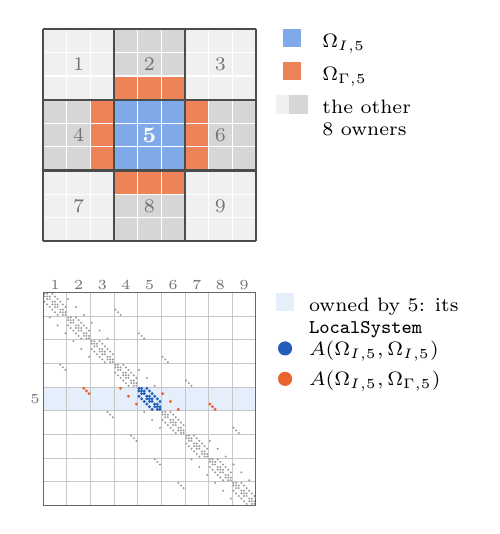
\begin{tikzpicture}[x=1mm,y=1mm]
      \pgfmathsetmacro\mcs{27/9}   % cell of the mesh
      \pgfmathsetmacro\mh{27/81}   % entry of the matrix
      % mesh: 9 x 9 cells, 9 subdomains of 3 x 3 cells, subdomain 5 in the centre
      \begin{scope}[shift={(0,33.5)}]
        \foreach \x in {0,...,8} {
          \foreach \y in {0,...,8} {
            \pgfmathtruncatemacro\sx{floor(\x/3)}
            \pgfmathtruncatemacro\sy{floor(\y/3)}
            \pgfmathtruncatemacro\own{(\sx==1)&&(\sy==1)}
            \pgfmathtruncatemacro\ovl{((\x>=3)&&(\x<=5)&&((\y==2)||(\y==6)))||((\y>=3)&&(\y<=5)&&((\x==2)||(\x==6)))}
            \pgfmathtruncatemacro\chk{mod(\sx+\sy,2)}
            \ifnum\own=1 \def\fc{schwarz!60}%
            \else\ifnum\ovl=1 \def\fc{gamg!80}%
            \else\ifnum\chk=0 \def\fc{black!6}\else\def\fc{black!16}\fi\fi\fi
            \fill[\fc] (\x*\mcs,\y*\mcs) rectangle ++(\mcs,\mcs);
          }}
        \draw[white,line width=0.4pt] (0,0) grid[step=\mcs] (27,27);
        \foreach \k in {0,3,6,9} {
          \draw[black!70,line width=0.8pt] (\k*\mcs,0) -- (\k*\mcs,27);
          \draw[black!70,line width=0.8pt] (0,\k*\mcs) -- (27,\k*\mcs);
        }
        \foreach \s in {1,...,9} {   % numbers: row-major from the top left, as the blocks of the matrix
          \pgfmathsetmacro\cx{(mod(\s-1,3)*3+1.5)*\mcs}
          \pgfmathsetmacro\cy{(2-floor((\s-1)/3))*3*\mcs+1.5*\mcs}
          \ifnum\s=5 \node[font=\footnotesize\bfseries,text=white] at (\cx,\cy) {5};
          \else \node[font=\scriptsize,text=black!55] at (\cx,\cy) {\s};\fi
        }
      \end{scope}
      \node[anchor=north west,font=\scriptsize,align=left,inner sep=0pt] at (29.5,60.5) {%
        \begin{tabular}{@{}c@{\ \ }>{\raggedright\arraybackslash}p{19mm}@{}}
          \textcolor{schwarz!60}{\rule{2.3mm}{2.3mm}} & $\Omega_{I,5}$\\[3pt]
          \textcolor{gamg!80}{\rule{2.3mm}{2.3mm}}    & $\Omega_{\Gamma,5}$\\[3pt]
          \textcolor{black!6}{\rule{2.3mm}{2.3mm}}\hspace{-0.6mm}\textcolor{black!16}{\rule{2.3mm}{2.3mm}} & the other\newline 8 owners\\
        \end{tabular}};
      % matrix 81 x 81: unknowns numbered subdomain by subdomain
      \begin{scope}[shift={(0,27)}]
        \fill[schwarz!12] (0,-36*\mh) rectangle (27,-45*\mh);          % rows owned by 5
        \foreach \k in {1,...,8} {
          \draw[black!22,line width=0.25pt] (\k*9*\mh,0) -- (\k*9*\mh,-27);
          \draw[black!22,line width=0.25pt] (0,-\k*9*\mh) -- (27,-\k*9*\mh);
        }
        \foreach \x in {0,...,8} {
          \foreach \y in {0,...,8} {
            \pgfmathtruncatemacro\rr{9*(3*(2-floor(\y/3))+floor(\x/3))+3*(2-mod(\y,3))+mod(\x,3)}
            \pgfmathtruncatemacro\rb{floor(\rr/9)}
            \foreach \dx/\dy in {0/0,1/0,-1/0,0/1,0/-1} {
              \pgfmathtruncatemacro\nx{\x+\dx}
              \pgfmathtruncatemacro\ny{\y+\dy}
              \pgfmathtruncatemacro\inside{(\nx>=0)&&(\nx<=8)&&(\ny>=0)&&(\ny<=8)}
              \ifnum\inside=1
                \pgfmathtruncatemacro\cc{9*(3*(2-floor(\ny/3))+floor(\nx/3))+3*(2-mod(\ny,3))+mod(\nx,3)}
                \pgfmathtruncatemacro\cb{floor(\cc/9)}
                \ifnum\rb=4
                  \ifnum\cb=4 \def\dc{schwarz!85!black}\else\def\dc{gamg}\fi
                  \fill[\dc] ({(\cc+0.5)*\mh},{-(\rr+0.5)*\mh}) circle (0.62*\mh);
                \else
                  \fill[black!40] ({(\cc+0.5)*\mh},{-(\rr+0.5)*\mh}) circle (0.42*\mh);
                \fi
              \fi
            }
          }}
        \draw[black!60,line width=0.4pt] (0,0) rectangle (27,-27);
        \foreach \s in {1,...,9} \node[font=\tiny,text=black!55,above,inner sep=1pt] at ({(9*\s-4.5)*\mh},0) {\s};
        \node[font=\tiny,text=black!55,left,inner sep=1pt] at (0,{-40.5*\mh}) {5};
      \end{scope}
      \node[anchor=north west,font=\scriptsize,align=left,inner sep=0pt] at (29.5,27) {%
        \begin{tabular}{@{}c@{\ \ }>{\raggedright\arraybackslash}p{19mm}@{}}
          \textcolor{schwarz!12}{\rule{2.3mm}{2.3mm}} & owned by 5: its \code{LocalSystem}\\[3pt]
          \tikz\fill[schwarz!85!black] (0,0) circle (0.9mm); & $A(\Omega_{I,5},\Omega_{I,5})$\\[3pt]
          \tikz\fill[gamg] (0,0) circle (0.9mm); & $A(\Omega_{I,5},\Omega_{\Gamma,5})$\\
        \end{tabular}};
    \end{tikzpicture}
  \end{columns}
\end{frame}

\begin{frame}{1. Introduction: Coarse Correction}
  \small
  \setlength{\parskip}{4pt}
  Given $R_0\in\R^{n_0\times n}$ whose rows span a coarse space of dimension $n_0\ll n$, and $A_{00}=R_0AR_0^\top$:
  \begin{align*}
    M^{-1}_{\star,\mathrm{additive}} &= R_0^\top A_{00}^{-1}R_0 + M^{-1}_{\star},\\[2pt]
    M^{-1}_{\star,\mathrm{deflated}} &= R_0^\top A_{00}^{-1}R_0 + M^{-1}_{\star}\left(I-AR_0^\top A_{00}^{-1}R_0\right),
    \qquad \star\in\{\mathrm{ASM},\mathrm{RAS}\}.
  \end{align*}

  \textbf{\color{schwarz}Deflated}: coarse correction first, then the local solves on the \alert{deflated residual}
  $r-Ax_0$, $x_0=R_0^\top A_{00}^{-1}R_0r$: one extra product with $A$.

  \textbf{\color{schwarz}Default} here, as in the experiments of the paper: \alert{RAS + deflated}.

  \vspace{2mm}
  \begin{block}{Key idea of the paper}
    $R_0$ is built \alert{algebraically}, from local generalized eigenproblems that only use entries of $A$:
    $A_{ii}$, $D_i$ and a lumped splitting $\At_{ii}$. No mesh, no near-kernel vectors, no Neumann matrices
    from a finite element assembly.
  \end{block}
\end{frame}

\begin{frame}{1. Introduction: Local Block Splitting}
  \small
  \begin{columns}[c,onlytextwidth]
    \column{0.58\textwidth}
    \setlength{\parskip}{3pt}
    \textbf{\color{schwarz}Lumping in the overlap.} Local ordering $[\Omega_{I,i},\Omega_{\Gamma,i},\Omega^c_i]$:
    the absolute row sums $s_i$ of $A(\Omega_{\Gamma,i},\Omega^c_i)$, i.e.\ the couplings of the overlap with the
    \alert{outside}, are taken off the diagonal of the overlap block:
    \vspace{-1mm}
    \[
      \At_{ii}=\begin{pmatrix} A_{I,i} & A_{I\Gamma,i}\\ A_{\Gamma I,i} & A_{\Gamma,i}-\mathrm{diag}(s_i)\end{pmatrix}
    \]
    \vspace{-3mm}

    Only the \alert{diagonal of the overlap block} changes: $O(n_i)$, no communication
    once the overlap rows are known.

    % block structure of the local matrices
    \column{0.40\textwidth}
    \centering
    \vspace{1mm}
    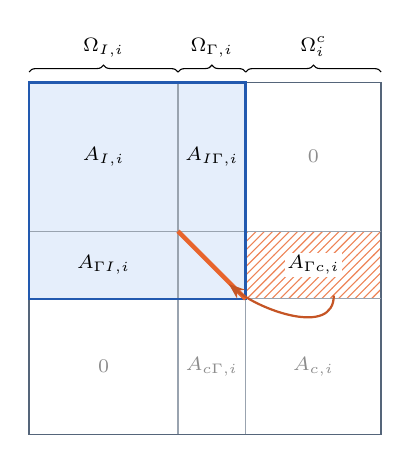
\begin{tikzpicture}[x=0.86mm,y=0.86mm,font=\scriptsize]
      % blocks: I = 0..22, Gamma = 22..32, c = 32..52
      \fill[schwarz!12] (0,52) rectangle (32,20);
      \fill[pattern=north east lines,pattern color=gamg!80] (32,30) rectangle (52,20);
      \draw[boxedge,line width=0.5pt] (0,0) rectangle (52,52);
      \foreach \t in {22,32} {\draw[boxedge!60] (\t,0) -- (\t,52); \draw[boxedge!60] (0,52-\t) -- (52,52-\t);}
      \draw[schwarz!80!black,line width=1pt] (0,52) rectangle (32,20);
      \draw[gamg,line width=1.6pt] (22,30) -- (32,20);
      \node at (11,41) {$A_{I,i}$}; \node at (27,41) {$A_{I\Gamma,i}$};
      \node at (11,25) {$A_{\Gamma I,i}$};
      \node[fill=white,inner sep=0.8pt] at (42,25) {$A_{\Gamma c,i}$};
      \node[text=black!45] at (42,10) {$A_{c,i}$}; \node[text=black!45] at (42,41) {$0$}; \node[text=black!45] at (11,10) {$0$};
      \node[text=black!45] at (27,10) {$A_{c\Gamma,i}$};
      \draw[decorate,decoration={brace,amplitude=2.5pt}] (0,53.5) -- (22,53.5) node[midway,above=2pt] {$\Omega_{I,i}$};
      \draw[decorate,decoration={brace,amplitude=2.5pt}] (22,53.5) -- (32,53.5) node[midway,above=2pt] {$\Omega_{\Gamma,i}$};
      \draw[decorate,decoration={brace,amplitude=2.5pt}] (32,53.5) -- (52,53.5) node[midway,above=2pt] {$\Omega^c_i$};
      \draw[-{Stealth[length=2mm]},gamg!85!black,line width=0.8pt] (45,20.5) to[out=-90,in=-40] (29.5,22.2);
    \end{tikzpicture}\\[2mm]
    {\scriptsize
    \begin{tabular}{@{}c@{\ \ }>{\raggedright\arraybackslash}p{42mm}@{}}
      \tikz\draw[schwarz!80!black,line width=1pt] (0,0) rectangle (2.3mm,2.3mm); & $A_{ii}$; $\At_{ii}$ is the same block,\newline except the orange diagonal\\[3pt]
      \tikz\fill[pattern=north east lines,pattern color=gamg!80] (0,0) rectangle (2.3mm,2.3mm); &
        $A_{\Gamma c,i}$: its absolute row sums give $s_i$\\[3pt]
      \tikz[baseline=-0.5ex]\draw[gamg,line width=1.6pt] (0,-1.1mm) -- (2.3mm,1.1mm); & diagonal of $A_{\Gamma,i}$: $-\,\mathrm{diag}(s_i)$\\
    \end{tabular}}
  \end{columns}
\end{frame}

\begin{frame}{1. Introduction: Coarse Space}
  \small
  \begin{columns}[T,onlytextwidth]
    \column{0.58\textwidth}
    \setlength{\parskip}{3pt}
    \textbf{\color{schwarz}Local eigenproblem.} $B_i=D_iA_{ii}D_i$, $L_i=\ker B_i$, $K_i=\ker\At_{ii}$, $\Pi_i$
    projection onto $\mathrm{range}(\At_{ii})$. Find
    $(\lambda,u)\in\mathbb{C}\times\mathbb{C}^{n_i}$ s.t.: $\Pi_iB_i\Pi_i\,u=\lambda\,\At_{ii}\,u$

    \textbf{\color{schwarz}Coarse space.} $Z_i$ spans
    \vspace{-1.5mm}
    \[
      \underbrace{(L_i\cap K_i)^{\perp_{K_i}}}_{\text{infinite eigenvalues}}\ \oplus\
      \mathrm{span}\left\{u:\ |\lambda|\ge 1/\tau\right\}
    \]
    \vspace{-3.5mm}

    Modes with high $|\lambda|$ are selected: the local correction does not effectively reduce 
    their error components; represented in the coarse space: $R_0^\top=[R_1^\top D_1Z_1,\dots,R_N^\top D_NZ_N]$
    

    % spectrum + selected modes of subdomain 5
    \column{0.40\textwidth}
    \vspace{1mm}
    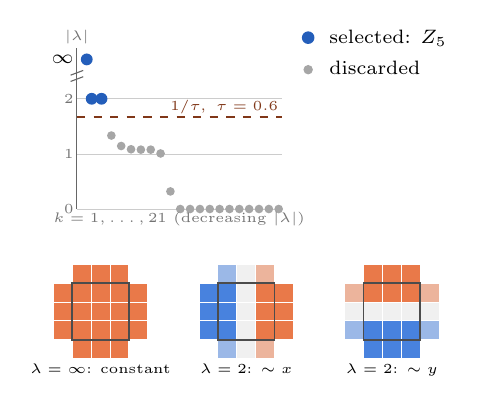
\begin{tikzpicture}[x=1mm,y=1mm]
      % ---- spectrum of the local eigenproblem of subdomain 5 (example of the previous slides), tau = 0.6
      \begin{scope}[shift={(3,22)}]
        \pgfmathsetmacro\ly{7}     % mm per unit of lambda
        \draw[black!20,line width=0.25pt] (0,0) -- (26,0) (0,\ly) -- (26,\ly) (0,2*\ly) -- (26,2*\ly);
        \draw[black!60,line width=0.4pt] (0,0) -- (0,20.5);
        \foreach \v in {0,1,2} \node[font=\tiny,text=black!55,left,inner sep=1pt] at (0,\v*\ly) {\v};
        \node[font=\scriptsize,left,inner sep=1pt] at (0,19) {$\infty$};
        \node[font=\tiny,text=black!55,above,inner sep=1pt] at (0,20.5) {$|\lambda|$};
        \draw[black!60,line width=0.4pt] (-0.8,16.2) -- (0.8,16.8) (-0.8,17.0) -- (0.8,17.6);   % axis break
        \draw[gamg!55!black,dashed,line width=0.6pt] (0,1.667*\ly) -- (26,1.667*\ly)
          node[font=\tiny,text=gamg!55!black,above left,inner sep=1pt] {$1/\tau,\ \tau=0.6$};
        \fill[schwarz!85!black] (1.25,19) circle (0.75);
        \foreach \k/\l in {2/2,3/2,4/1.333,5/1.143,6/1.084,7/1.077,8/1.077,9/1.008,10/0.319,
                           11/0,12/0,13/0,14/0,15/0,16/0,17/0,18/0,19/0,20/0,21/0} {
          \pgfmathsetmacro\xx{(\k-0.5)*1.25}
          \pgfmathparse{\l>=1.667}
          \ifnum\pgfmathresult=1 \fill[schwarz!85!black] (\xx,\l*\ly) circle (0.75);
          \else \fill[black!35] (\xx,\l*\ly) circle (0.55);\fi
        }
        \node[font=\tiny,text=black!55,below,inner sep=1pt] at (13,0) {$k=1,\dots,21$ (decreasing $|\lambda|$)};
      \end{scope}
      \node[anchor=north west,font=\scriptsize,align=left,inner sep=0pt] at (31.5,45) {%
        \begin{tabular}{@{}c@{\ \ }>{\raggedright\arraybackslash}p{17mm}@{}}
          \tikz\fill[schwarz!85!black] (0,0) circle (0.8mm); & selected: $Z_5$\\[3pt]
          \tikz\fill[black!35] (0,0) circle (0.6mm); & discarded\\
        \end{tabular}\\[2mm]
       };
      % ---- the three selected modes on Omega_5 (cells of the cross); framed: Omega_I, where D_5 u is kept
      \pgfmathsetmacro\ec{2.4}
      \colorlet{cbase}{black!6}
      \foreach \m/\lab/\vals in {%
          0/{$\lambda=\infty$: constant}/{3/5/1,4/5/1,5/5/1,3/4/1,4/4/1,5/4/1,3/3/1,4/3/1,5/3/1,3/6/1,4/6/1,5/6/1,2/5/1,2/4/1,2/3/1,6/5/1,6/4/1,6/3/1,3/2/1,4/2/1,5/2/1},
          1/{$\lambda=2$: $\sim x$}/{3/5/-1,4/5/0,5/5/1,3/4/-1,4/4/0,5/4/1,3/3/-1,4/3/0,5/3/1,3/6/-0.5,4/6/0,5/6/0.5,2/5/-1,2/4/-1,2/3/-1,6/5/1,6/4/1,6/3/1,3/2/-0.5,4/2/0,5/2/0.5},
          2/{$\lambda=2$: $\sim y$}/{3/5/1,4/5/1,5/5/1,3/4/0,4/4/0,5/4/0,3/3/-1,4/3/-1,5/3/-1,3/6/1,4/6/1,5/6/1,2/5/0.5,2/4/0,2/3/-0.5,6/5/0.5,6/4/0,6/3/-0.5,3/2/-1,4/2/-1,5/2/-1}} {
        \begin{scope}[shift={(\m*18.5,3)}]
          \foreach \x/\y/\v in \vals {
            \pgfmathtruncatemacro\p{round(abs(\v)*85)}
            \pgfmathparse{\v<0}
            \ifnum\pgfmathresult=1 \def\fc{schwarz!\p!cbase}\else\def\fc{gamg!\p!cbase}\fi
            \fill[\fc] ({(\x-2)*\ec},{(\y-2)*\ec}) rectangle ++(\ec,\ec);
          }
          \draw[white,line width=0.3pt] (\ec,0) grid[step=\ec] (4*\ec,5*\ec) (0,\ec) grid[step=\ec] (5*\ec,4*\ec);
          \draw[black!70,line width=0.6pt] (\ec,\ec) rectangle (4*\ec,4*\ec);
          \node[font=\tiny,anchor=north,inner sep=1pt] at (2.5*\ec,-0.3) {\lab};
        \end{scope}
      }
    \end{tikzpicture}
  \end{columns}
  
  \vspace{2mm}
  \colorbox{schwarz!14}{\parbox{\dimexpr\linewidth-6pt}{\footnotesize\textbf{Bound} for $M^{-1}_{\mathrm{ASM,add}}$, SPD and diag.\ dominant $A$}}\par\nointerlineskip
  \colorbox{schwarz!5}{\parbox{\dimexpr\linewidth-6pt}{\footnotesize\centering
    $\kappa\left(M^{-1}A\right)\le(k_c+1)\left(2+(2k_c+1)\,k_m/\tau\right)$\\[2pt]
    \raggedright\scriptsize $k_c$: colours of the subdomain graph, $k_m$: max subdomains per row;
    independent of $N$ and of the coefficients.}}

\end{frame}

% =============================================================================================
\section{Code structure}
% =============================================================================================

\begin{frame}{2. Code structure: modules}
  \begin{columns}[T,onlytextwidth]
    \column{\textwidth}
    \centering
    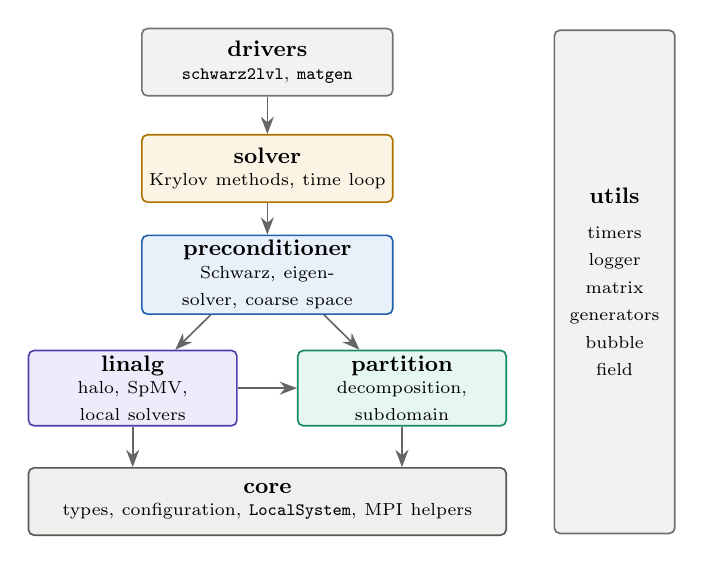
\begin{tikzpicture}[x=1mm,y=1mm,scale=0.9,every node/.append style={transform shape}]
      \node[md,draw=black!55,fill=black!5] (drv) at (0,0)  {\textbf{drivers}\\[-2pt]\scriptsize\texttt{schwarz2lvl}, \texttt{matgen}};
      \node[md,mod=solv] (solv) at (0,-15) {\textbf{solver}\\[-2pt]\scriptsize Krylov methods, time loop};
      \node[md,mod=prec] (prec) at (0,-30) {\textbf{preconditioner}\\[-2pt]\scriptsize Schwarz, eigensolver, coarse space};
      \node[md=28mm,mod=linalg] (lin) at (-19,-46) {\textbf{linalg}\\[-2pt]\scriptsize halo, SpMV, local solvers};
      \node[md=28mm,mod=part] (part) at (19,-46) {\textbf{partition}\\[-2pt]\scriptsize decomposition, subdomain};
      \node[md=66mm,mod=core] (core) at (0,-62) {\textbf{core}\\[-2pt]\scriptsize types, configuration, \texttt{LocalSystem}, MPI helpers};
      \node[rounded corners=2pt,font=\small,align=center,minimum width=17mm,minimum height=71mm,inner sep=2pt,mod=utils,line width=0.6pt] (utils) at (49,-31)
        {\textbf{utils}\\[3pt]\scriptsize timers\\ \scriptsize logger\\ \scriptsize matrix\\ \scriptsize generators\\ \scriptsize bubble\\ \scriptsize field};
      \draw[dep] (drv) -- (solv);
      \draw[dep] (solv) -- (prec);
      \draw[dep] ($(prec.south)+(-8,0)$) -- ($(lin.north)+(6,0)$);
      \draw[dep] ($(prec.south)+(8,0)$) -- ($(part.north)+(-6,0)$);
      \draw[dep] (lin) -- (part);
      \draw[dep] (lin.south) -- (lin.south |- core.north);
      \draw[dep] (part.south) -- (part.south |- core.north);
    \end{tikzpicture}
  \end{columns}
  
  \small
  \vspace{5mm}
  \muted{The colours of the modules are kept in every class diagram that follows.}
\end{frame}

\begin{frame}{2. Code structure: main classes}
  \cmfocus{all}
  \centering
  \vspace{-1mm}
  \mapsec\Wfull{0.97\textwidth}\\[0.6mm]
  {\scriptsize\muted{italic: abstract interface \quad
  \tikz[baseline=-0.6ex]\draw[inh] (0,0)--(5mm,0); inheritance \quad
  \tikz[baseline=-0.6ex]\draw[comp] (0,0)--(6mm,0); owns (\texttt{unique\_ptr}) \quad
  \tikz[baseline=-0.6ex]\draw[use] (0,0)--(6mm,0); uses \quad
  \tikz[baseline=-0.6ex]\draw[flow] (0,0)--(6mm,0); data passed on}}
\end{frame}

\begin{frame}[fragile]{2. Code structure: flow of a solve}
  
  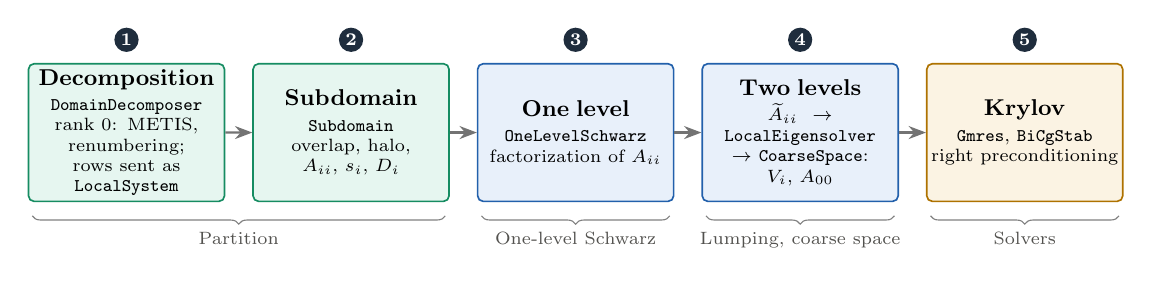
\begin{tikzpicture}[x=1mm,y=1mm,scale=0.92,every node/.append style={transform shape},
      st/.style={rounded corners=2pt,text width=26mm,minimum height=19mm,align=center,font=\scriptsize,inner sep=1.5pt,line width=0.6pt},
      ar/.style={-{Stealth[length=2.2mm]},line width=0.8pt,draw=black!55},
      num/.style={circle,fill=titlebg,text=white,font=\scriptsize\bfseries,inner sep=1.1pt}]
    \node[st,mod=part]   (s1) at (0,0)   {\textbf{\small Decomposition}\\[2pt]{\ttfamily DomainDecomposer}\\ rank 0: METIS, renumbering;\\ rows sent as \texttt{LocalSystem}};
    \node[st,mod=part]   (s2) at (31,0)  {\textbf{\small Subdomain}\\[2pt]{\ttfamily Subdomain}\\ overlap, halo,\\ $A_{ii}$, $s_i$, $D_i$};
    \node[st,mod=prec]   (s3) at (62,0)  {\textbf{\small One level}\\[2pt]{\ttfamily OneLevelSchwarz}\\ factorization of $A_{ii}$};
    \node[st,mod=prec]   (s4) at (93,0)  {\textbf{\small Two levels}\\[2pt]$\widetilde A_{ii}\to$ {\ttfamily LocalEigensolver}\\ $\to$ {\ttfamily CoarseSpace}: $V_i$, $A_{00}$};
    \node[st,mod=solv]   (s5) at (124,0) {\textbf{\small Krylov}\\[2pt]{\ttfamily Gmres}, {\ttfamily BiCgStab}\\ right preconditioning};
    \foreach \a/\b in {s1/s2,s2/s3,s3/s4,s4/s5} \draw[ar] (\a) -- (\b);
    \foreach \n/\k in {s1/1,s2/2,s3/3,s4/4,s5/5} \node[num] at ($(\n.north)+(0,3.2)$) {\k};
    \draw[decorate,decoration={brace,mirror,amplitude=3pt},black!50] (-13,-11.5) -- (44,-11.5) node[midway,below=3pt,font=\scriptsize,text=ink2] {Partition};
    \draw[decorate,decoration={brace,mirror,amplitude=3pt},black!50] (49,-11.5) -- (75,-11.5) node[midway,below=3pt,font=\scriptsize,text=ink2] {One-level Schwarz};
    \draw[decorate,decoration={brace,mirror,amplitude=3pt},black!50] (80,-11.5) -- (106,-11.5) node[midway,below=3pt,font=\scriptsize,text=ink2] {Lumping, coarse space};
    \draw[decorate,decoration={brace,mirror,amplitude=3pt},black!50] (111,-11.5) -- (137,-11.5) node[midway,below=3pt,font=\scriptsize,text=ink2] {Solvers};
  \end{tikzpicture}
  
  \vspace{2mm}
  After step 1 \alert{no process holds global data}: every global operation is a reduction, a
          neighbour exchange, or the assembly of $A_{00}$.
  
  \alert{One MPI process} = one subdomain. Every phase is timed (\code{ScopedTimer}: min / avg / max over the ranks).
  
\end{frame}

% =============================================================================================
\section{Partition}
% =============================================================================================

\begin{frame}[fragile]{3. Partition: decomposition}
  \cmfocus{DomainDecomposer,MatrixMarketIO,GraphPartitioner,LocalSystem}
  %\mapbadge\Wpart
  \begin{columns}[c,onlytextwidth]
    \column{0.6\textwidth}
      \small
      \code{DomainDecomposer::decompose}, as OpenFOAM \code{decomposePar}: all global work on rank 0, once.
      \begin{enumerate}
        \item Read a Matrix Market file or run a generator.
        \item METIS k-way on $\mathcal{G}(A+A^\top)$, fixed seed.
        \item Renumber: rank $p$ owns the \alert{contiguous} range $[o_p,o_{p+1})$.
        \item Send every rank \alert{only its rows} (CSR, global columns).
      \end{enumerate}
    \column{0.36\textwidth}
\begin{lstlisting}
struct LocalSystem { // per rank
  MPI_Comm comm;
  GlobalIndex n_global;
  std::vector<GlobalIndex>
  ownership, // [o_p, o_p+1)
  row_ptr, col; // owned rows
  std::vector<Scalar> val, rhs;
  int  block_size; // per cell
  bool symmetric;
};
\end{lstlisting}  
    \end{columns}
    \vspace{2mm}
  \textbf{\color{schwarz}Result}: \code{LocalSystem} = what an OpenFOAM processor owns: \code{lduMatrix} + \code{globalIndex}.
  \vspace{2mm}\begin{center}\mapsec\Wpart{0.66\textwidth}\end{center}
\end{frame}

\begin{frame}{3. Partition: subdomain}
  \cmfocus{Subdomain,HaloExchange,DistributedMatrix,LocalSystem}
  %\mapbadge\Wpart
  \small
  \code{Subdomain(const LocalSystem\&, pou)}: each rank builds its own overlapping subdomain, collectively,
  \alert{without global data}.
  \begin{columns}[T,onlytextwidth]
    \column{0.49\textwidth}
    \begin{enumerate}
      \item \textbf{Overlap} $\Omega_{\Gamma,i}$: off-process columns of the owned rows, plus remote rows with a
            column in $\Omega_{I,i}$ (one \code{Alltoall} + one \code{Alltoallv}).
      \item \textbf{Halo} pattern $\to$ \code{HaloExchange}.
      \item \textbf{Ghost rows} $A(\Omega_{\Gamma,i},:)$ from their owners.
    \end{enumerate}
    \column{0.49\textwidth}
    \begin{enumerate}\setcounter{enumi}{3}
      \item \textbf{Local matrices} $A_{ii}$ (col-major) and $A(\Omega_{I,i},\Omega_i)$ (row-major);
            \alert{lumping sums} $s_i$ while ghost rows arrive.
      \item \textbf{Partition of unity}: Default is \code{bool}, $D_i=1$ on $\Omega_{I,i}$, $0$ on $\Omega_{\Gamma,i}$.
    \end{enumerate}
  \end{columns}
  \vfill
  \begin{center}\mapsec\Wpart{0.74\textwidth}\end{center}
\end{frame}

\begin{frame}[fragile]{3. Partition: halo exchange and distributed product}
  %\mapbadge\Wsub
  \centering
  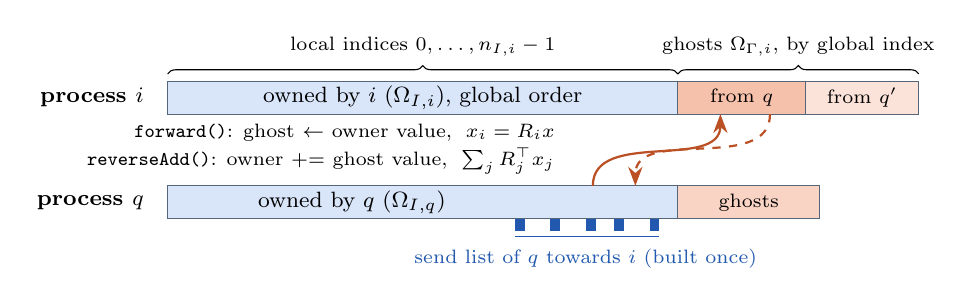
\begin{tikzpicture}[x=0.9mm,y=0.7mm]
    \fill[schwarz!18] (0,10) rectangle (72,16);
    \fill[gamg!40] (72,10) rectangle (90,16);
    \fill[gamg!18] (90,10) rectangle (106,16);
    \draw[boxedge] (0,10) rectangle (106,16);
    \draw[boxedge] (72,10) -- (72,16) (90,10) -- (90,16);
    \node[font=\footnotesize] at (36,13) {owned by $i$ ($\Omega_{I,i}$), global order};
    \node[font=\scriptsize] at (81,13) {from $q$};
    \node[font=\scriptsize] at (98,13) {from $q'$};
    \node[anchor=east,font=\footnotesize\bfseries] at (-2,13) {process $i$};
    \draw[decorate,decoration={brace,amplitude=3pt}] (0,17.3) -- (72,17.3)
         node[midway,above=3pt,font=\scriptsize] {local indices $0,\dots,n_{I,i}-1$};
    \draw[decorate,decoration={brace,amplitude=3pt}] (72,17.3) -- (106,17.3)
         node[midway,above=3pt,font=\scriptsize] {ghosts $\Omega_{\Gamma,i}$, by global index};
    \fill[schwarz!18] (0,-9) rectangle (72,-3);
    \fill[gamg!28] (72,-9) rectangle (92,-3);
    \draw[boxedge] (0,-9) rectangle (92,-3);
    \draw[boxedge] (72,-9) -- (72,-3);
    \node[font=\footnotesize] at (26,-6) {owned by $q$ ($\Omega_{I,q}$)};
    \node[font=\scriptsize] at (82,-6) {ghosts};
    \node[anchor=east,font=\footnotesize\bfseries] at (-2,-6) {process $q$};
    \foreach \x in {49,54,59,63,68} \fill[schwarz!80!black] (\x,-9) rectangle ++(1.4,-2.2);
    \draw[schwarz!80!black] (49,-12.2) -- (69.4,-12.2);
    \node[anchor=north,font=\scriptsize,schwarz!80!black] at (59,-12.6) {send list of $q$ towards $i$ (built once)};
    \draw[-{Stealth[length=2.4mm]},line width=0.8pt,gamg!80!black] (60,-3) to[out=90,in=-90] (78,10);
    \draw[-{Stealth[length=2.4mm]},line width=0.8pt,dashed,gamg!80!black] (85,10) to[out=-90,in=90] (66,-3);
    \node[anchor=east,font=\scriptsize] at (56,6.7) {\code{forward()}: ghost $\leftarrow$ owner value, \;$x_i = R_i x$};
    \node[anchor=east,font=\scriptsize] at (56,1.5) {\code{reverseAdd()}: owner $\mathrel{+}=$ ghost value, \;$\sum_j R_j^\top x_j$};
  \end{tikzpicture}
  \vspace{0.5mm}
  \begin{columns}[c,onlytextwidth]
    \column{0.50\textwidth}
    \small
    \textbf{\color{schwarz}Contiguous ownership}: the ghosts of one neighbour are a contiguous block, received
            in place (\code{MPI\_Irecv} into the vector).
    
    \textbf{\color{schwarz}Non-blocking point-to-point}, neighbours only; buffers reused.
    
    \textbf{\color{schwarz}\code{exchange<T>()}} for irregular data (ghost rows, sparse rows).
    
    \column{0.47\textwidth}
\begin{lstlisting}
// DistributedMatrix::apply = lduMatrix::Amul
void apply(const Vec& x, Vec& y) const {
  xloc_.head(sd_.nOwned()) = x;
  sd_.halo().forward(xloc_); // ghost values
  y.noalias() = sd_.Aowned() * xloc_;
}
\end{lstlisting}
  \end{columns}
\end{frame}

% =============================================================================================
\section{One-level Schwarz}
% =============================================================================================

\begin{frame}[fragile]{4. One-level Schwarz}
  \cmfocus{Preconditioner,OneLevelSchwarz,LocalSolver}
  %\mapbadge\Wone
  \begin{columns}[c,onlytextwidth]
    \column{0.63\textwidth}
\begin{lstlisting}
void OneLevelSchwarz::apply(const Vec& r, Vec& z) const {
  rloc_.head(nI) = r;
  sd_.halo().forward(rloc_);          // R_i r
  solver_->solve(rloc_, yloc_);       // A_ii^{-1} R_i r
  if (variant_ == Variant::RAS) {
    yloc_.array() *= sd_.pou().array(); // D_i ...
    if (!sd_.booleanPou()) sd_.halo().reverseAdd(yloc_);
  } else
    sd_.halo().reverseAdd(yloc_);     // sum_j R_j^T ...
  z = yloc_.head(nI);
}
\end{lstlisting}
    \small
    Vectors hold \alert{owned entries only}; the overlap lives in work vectors.
    
    \textbf{\color{schwarz}Boolean PoU} (default): RAS needs \alert{one} \code{forward()}, no reverse communication.
    
    \column{0.34\textwidth}
    \centering
    \mapsec\Wone{0.98\linewidth}
  \end{columns}
\end{frame}

\begin{frame}{4. One-level Schwarz: local solvers}
  \cmfocus{LocalSolver,EigenSolver,UmfpackSolver,PardisoSolver,AmgSolver,ChainSolver,OneLevelSchwarz}
  %\mapbadge\Wone
  \begin{columns}[T,onlytextwidth]
    \column{0.63\textwidth}
    \small
    \textbf{Strategy interface} \code{LocalSolver}: \code{factorize}, \code{refactorize} (symbolic analysis
    reused), multi-RHS \code{solve}, \code{solveTranspose}.
    
    \vspace{2mm}
    Backends chosen at run time: Eigen (SparseLU, LLT, LDLT), UMFPACK, MKL PARDISO, one AMGCL V-cycle.
    
    \vspace{2mm}
    Built by a \alert{factory}, \code{makeLocalSolver(spec)}: backend, factorization, symmetry, precision.
    
    \vspace{2mm}
    \code{ChainSolver}: Cholesky $\to$ LDL$^\top\to$ LU, keeps the first that works
            (symmetric only if $A$ is \emph{known} to be symmetric).
    
            \vspace{2mm}
    Precision as a \alert{template parameter}; \code{if constexpr} removes the conversions in the
            \code{double} instantiation.
    
    \column{0.34\textwidth}
    \centering
    \mapsec\Wone{0.98\linewidth}
  \end{columns}
  
  \begin{exampleblock}{On G100}
    \footnotesize PARDISO runs 2 steps of iterative refinement per solve: disabled
    $\Rightarrow$ \textbf{3--3.7$\times$} faster, same iterations.
  \end{exampleblock}
\end{frame}

% =============================================================================================
\section{Lumping \& local block splitting}
% =============================================================================================

\begin{frame}[fragile]{5. Lumping \& local block splitting}
  \cmfocus{BlockSplitting,LocalEigensolver,TwoLevelSchwarz}
  %\mapbadge\Wlump
  \begin{columns}[T,onlytextwidth]
    \column{0.56\textwidth}
\begin{lstlisting}
SpMat buildLocalBlockSplitting(const Subdomain& sd) {
  SpMat At = sd.Aii();
  const Vec& s = sd.lumpingSums();  // from Subdomain
  for (LocalIndex j = 0; j < sd.nGhost(); ++j) {
    const LocalIndex l = sd.nOwned() + j;
    At.coeffRef(l, l) -= s[j]; // A_Gamma - diag(s)
  }
  At.makeCompressed();
  return At;
}
\end{lstlisting}
    \column{0.41\textwidth}
    \centering
    \mapsec\Wlump{0.98\linewidth}\\[2mm]
  
  \end{columns}
  
  \small  
  $s_i(j)=\sum_{k\notin\Omega_i}|A(j,k)|$: summed by \code{Subdomain}; the outside of $\Omega_i$ is never stored.

  \begin{block}{Consequence for the eigensolver}
    \small Zero row sums of $A$ give $\widetilde A_{ii}\mathbf{1}=0$ on
    floating subdomains: $\widetilde A_{ii}$ is \alert{singular}, it cannot be factorized as it is.
  \end{block}          
\end{frame}

% =============================================================================================
\section{Coarse space: eigenvalue problem}
% =============================================================================================

\begin{frame}{6. Coarse space: the local eigensolver}
  \cmfocus{LocalEigensolver,ProjectedOperator,BlockSplitting}
  %\mapbadge\Weig
  \small
  \begin{columns}[T,onlytextwidth]
    \column{0.5\textwidth}
    \code{LocalEigensolver::compute(}$A_{ii}$, $\widetilde A_{ii}$, $D_i$\code{)} $\to Z_i$:
    \begin{enumerate}
      \item Factorize $\widetilde A_{ii}+\sigma I$, $\sigma=10^{-13}\|\widetilde A_{ii}\|$.
      \item \textbf{Kernel} $K_i$: block inverse iteration (multi-RHS solves) + SVD; left kernel by
            transposed solves if $A$ is non-symmetric.
      \item \textbf{Infinite eigenvalues}: $(L_i\cap K_i)^{\perp_{K_i}}$ computed \alert{exactly} from an SVD
            of $B_iQ$, $B_i=D_iA_{ii}D_i$.
    \end{enumerate}
    \column{0.5\textwidth}
    \begin{enumerate}
      \setcounter{enumi}{3}
      \item \textbf{Finite eigenvalues}: restarted Arnoldi (Spectra) on the matrix-free
            \code{ProjectedOperator}: $T=\Pi_K(\widetilde A_{ii}+\sigma I)^{-1}\Pi_RB_i\Pi_K$. 
            one SpMV + one pair of triangular solves. 
            
            \footnotesize
            \muted{Keep $|\lambda|\ge1/\tau$: with \texttt{nev}$\,\ge128$, start from $k=32$ and enlarge while 
            $|\lambda|\ge1/\tau$: the cost follows the \alert{selected} vectors.}
    \end{enumerate}
  \end{columns}
  \centering
  
  \vspace{3mm}
  \mapsec\Weig{0.4\linewidth}
\end{frame}

\begin{frame}{6. Coarse space: assembly of $A_{00}$ and coarse solvers}
  \cmfocus{CoarseSpace,CoarseSolver,Root,Mumps,CPardiso}
  %\mapbadge\Wcoarse
  \begin{columns}[c,onlytextwidth]
    \column{0.70\textwidth}
    \small
      \textbf{\color{schwarz}$V_i$} $=\mathrm{orth}(D_iZ_i)$ by column-pivoted QR: same span, dependent vectors dropped, better
            conditioned $A_{00}$. Rank $i$ owns its $m_i$ coarse unknowns.
      
      \vspace{2mm}
      \textbf{\color{schwarz}$A_{00}$} from \alert{local products} only, with $W=R_0^\top$ restricted to $\Omega_i$ (one exchange of sparse rows):
            \[
              A_{00}=\sum_{i=1}^N W(\Omega_{I,i},:)^\top\,A(\Omega_{I,i},\Omega_i)\,W(\Omega_i,:)
            \]
            \vspace{-4mm}

      \vspace{2mm}
      \textbf{\color{schwarz}Boolean PoU}: restriction $V_i^\top R_ir$ and prolongation are communication-free.
      
      \vspace{2mm}
      \textbf{\color{schwarz}\code{CoarseSolver}} gets distributed triplets: \code{Root} (gather, factorize on rank 0), \code{Mumps},
            \code{CPardiso} (MKL cluster solver).
   
    \column{0.27\textwidth}
    \centering
    \mapsec\Wcoarse{0.98\linewidth}
  \end{columns}
\end{frame}

\begin{frame}[fragile]{6. Coarse space: the two levels together}
  \cmfocus{TwoLevelSchwarz,OneLevelSchwarz,CoarseSpace,Preconditioner}
  %\mapbadge\Wtwo
  \begin{columns}[c,onlytextwidth]
    \column{0.60\textwidth}
    \small
    \textbf{Setup} (\code{TwoLevelSchwarz} constructor):
    \begin{enumerate}
      \item \code{OneLevelSchwarz}: factorization of $A_{ii}$;
      \item $\At_{ii}$ $\to$ \code{LocalEigensolver} $\to$ $Z_i$ (no communication);
      \item failures reduced over all ranks before throwing (no rank left hanging in a collective);
      \item \code{CoarseSpace}: $V_i$, $A_{00}$, coarse factorization.
    \end{enumerate}
    
    \vspace{2mm}
    \textbf{Application}, transcription of the deflated formula:
\begin{lstlisting}
coarse_->apply(r, x0_);   // x0 = R0^T A00^{-1} R0 r
A_.apply(x0_, w_);        // extra product of "deflated"
w_ = r - w_;
one_->apply(w_, z1_);     // M_RAS^{-1} (r - A x0)
z = x0_ + z1_;
\end{lstlisting}
    \column{0.37\textwidth}
    \centering
    \mapsec\Wtwo{0.98\linewidth}\\[2mm]
    {\footnotesize Per application: 2 halo updates (local solve, extra SpMV) + the coarse solve.}
  \end{columns}
\end{frame}

% =============================================================================================
\section{Solvers}
% =============================================================================================

\begin{frame}{7. Solvers: Krylov methods}
  \cmfocus{KrylovSolver,Gmres,BiCgStab,Preconditioner}
  %\mapbadge\Wsolv
  \centering
  \mapsec\Wsolv{0.62\textwidth}\\[1mm]
  \begin{columns}[c,onlytextwidth]
    \column{0.48\textwidth}
    \small
    \textbf{\code{Gmres}} (restarted, as in the paper)
    \begin{itemize}
      \item \alert{Right} preconditioning: the residual is $b-Ax$, the stopping test of Section 4.
      \item CGS2: the $j$ inner products of a pass in \alert{one} \code{MPI\_Allreduce}.
      \item Convergence accepted only if the \alert{true} residual agrees (10\%).
    \end{itemize}
    \column{0.48\textwidth}
    \small
    \textbf{\code{BiCgStab}} (added for the extras)
    \begin{itemize}
      \item The algorithm of OpenFOAM \code{PBiCGStab}, 4 fused reductions per step instead of 6.
      \item Stopping tests: $\|r\|_2/\|b\|_2$, or OpenFOAM's normalised residual (\code{relTol}, \code{tolerance}).
      \item Iteration = one application of $M^{-1}$ in both: counts compare directly.
    \end{itemize}
  \end{columns}
\end{frame}

\begin{frame}{7. Solvers: verification}
  \small
  Every distributed component is compared with a \alert{sequential reference} built from the global matrix;
  every check is reduced over the ranks. \code{make check}: every test on 1, 2 and 4 processes.
  \vspace{1mm}
  \begin{center}
  \footnotesize
  \begin{tabular}{@{}l>{\raggedright\arraybackslash}p{0.66\textwidth}@{}}
    \toprule
    Test & What is compared\\
    \midrule
    \code{test\_subdomain} & overlap, halo, $A_{ii}$, lumping sums, partition of unity, distributed SpMV\\
    \code{test\_preconditioner} & sparse vs dense eigensolver and kernels; RAS/ASM $\times$ deflated/additive vs a
                                  reference assembled on one process; GMRES\\
    \code{test\_factorization} & Cholesky / LDL$^\top$ / LU chains, single precision, every coarse solver\\
    \code{test\_reuse}, \code{test\_inexact} & refactorization vs fresh setup, reuse policy; AMG local solver \muted{(extras)}\\
    \code{test\_bicgstab}, \code{test\_stopping} & BiCGStab, OpenFOAM stopping test \muted{(extras)}\\
    \code{test\_warmstart}, \code{test\_bubbles} & warm start, bubble field shared with OpenFOAM \muted{(extras)}\\
    \bottomrule
  \end{tabular}
  \end{center}
  
  \vspace{2mm}
  \textbf{\color{schwarz}On G100} every job script builds its own binaries, runs the tests on the compute nodes and records
          the source hash and the loaded modules next to the results.
  
\end{frame}

% =============================================================================================
\section{Reproduction of the paper}
% =============================================================================================

\begin{frame}{8. Reproduction of the paper: setting}
  \small
  \begin{columns}[c,onlytextwidth]
    \column{0.48\textwidth}
    \textbf{\color{schwarz}Same as the paper}
    
    \vspace{1mm}
      RAS + deflated, right-preconditioned GMRES(30), $\mathrm{rtol}=10^{-8}$, $x_0=0$, random $b$.
    
    \vspace{1mm}  
      SuiteSparse matrices of Table 1, convection--diffusion (4.1).
    
    \vspace{3mm}
    \textbf{\color{schwarz}Different}
    
    \vspace{1mm}
      CINECA Galileo100: 240 processes (paper: 256--4096).
    
    \vspace{1mm}
      METIS (ParMETIS), PARDISO (MUMPS), Spectra (SLEPc).
    
    \vspace{1mm}
      (4.1): upwind finite volumes (SUPG, P1/P2 elements).
    
    \column{0.49\textwidth}
    \footnotesize
    \begin{tabular}{@{}>{\raggedright\arraybackslash}p{0.27\linewidth}>{\raggedright\arraybackslash}p{\dimexpr0.73\linewidth-2\tabcolsep\relax}@{}}
      \toprule
      Experiment & Outcome\\
      \midrule
      Fig.~2, $\tau$ & reproduced: $n_0$ within 15\% (26\% at $\tau=0.6$), iterations 9--29\% lower\\\addlinespace[2pt]
      Table~1 & $n_0/N$ within 15\% on 8 of 10 matrices, iterations $\pm1$ on 6\\\addlinespace[2pt]
      Fig.~4, strong scaling & iterations bounded in $N$: $16\to12$ (paper $28\to15$)\\\addlinespace[2pt]
      Table~2 & 2D and 3D with $\nu\ge10^{-2}$; 3D, $\nu\le10^{-3}$: smaller $n_0$, more iterations\\\addlinespace[2pt]
      Failure & circuit5M\_dc: setup $>20$ min\\
      \bottomrule
    \end{tabular}
  \end{columns}
\end{frame}

\begin{frame}{8. Reproduction of the paper: Table 1}
  \begin{columns}[c,onlytextwidth]
    \column{0.52\textwidth}
    \footnotesize
    \begin{tabular}{@{}lrrrrr@{}}
      \toprule
      & \multicolumn{2}{c}{Paper} & \multicolumn{2}{c}{This work} & RAS\\
      \cmidrule(lr){2-3}\cmidrule(lr){4-5}
      Matrix & its & $n_0/N$ & its & $n_0/N$ & its\\
      \midrule
      finan512    & 6  & 10  & 6  & 22  & 6\\
      nxp1        & 20 & 77  & \color{gamg}29 & 95  & n.c.\\
      CoupCons3D  & 20 & 113 & 21 & 98  & 23\\
      tmt\_unsym  & 6  & 129 & 5  & 128 & n.c.\\
      ecology2    & 6  & 133 & 5  & 130 & n.c.\\
      thermal2    & 26 & 157 & \color{schwarz}5  & 139 & n.c.\\
      atmosmodj   & 7  & 298 & \color{gamg}14 & 286 & 79\\
      G3\_circuit & 8  & 279 & 7  & 279 & n.c.\\
      Transport   & 9  & 300 & 8  & 300 & n.c.\\
      memchip     & 36 & 226 & \color{schwarz}8  & 224 & 44\\
      \bottomrule
    \end{tabular}\par\vspace{1mm}
    {\scriptsize\muted{240 processes, \texttt{nev}$=300$, $\tau=0.9$. n.c.: not converged in 200 iterations.}}
    \column{0.45\textwidth}
    \small
    \begin{itemize}
      \item The paper states $\tau=0.6$, but its G3\_circuit row (8 its, $n_0=71\,385$) is the $\tau=0.9$
            point of its own Fig.~2 $\Rightarrow$ compared at \alert{$\tau=0.9$}.
      \item Wherever one-level RAS fails, the two-level method converges.
      \item Non-symmetric matrices: iterations also depend on the partition and on the random $b$
            (both differ between the codes).
    \end{itemize}
  \end{columns}
\end{frame}

\begin{frame}{8. Reproduction of the paper: effect of $\tau$ (Fig.~2, G3\_circuit)}
  \begin{columns}[c,onlytextwidth]
    \column{0.56\textwidth}
    \centering
    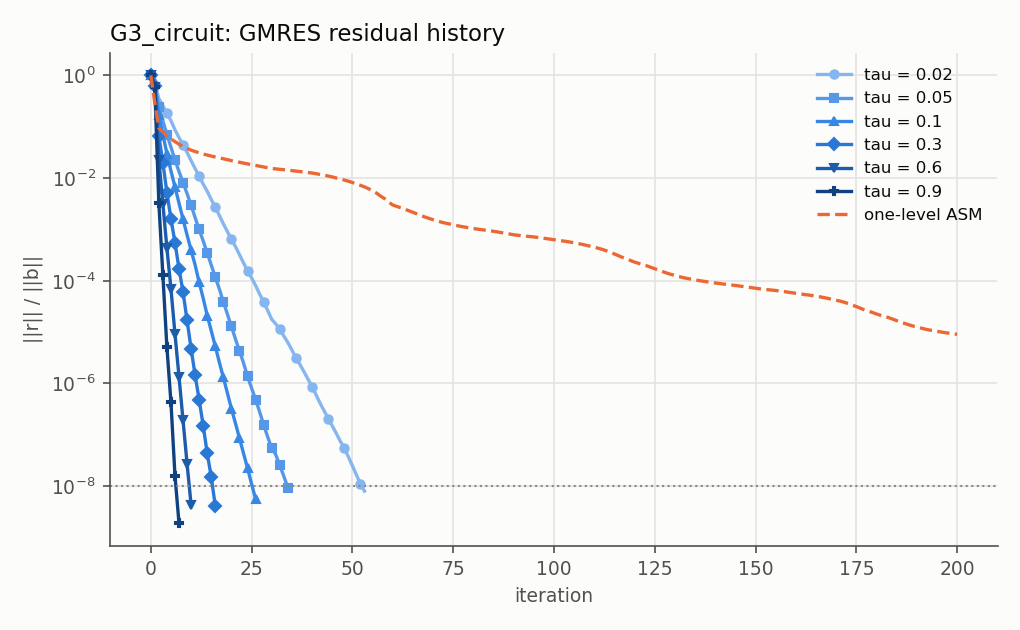
\includegraphics[width=\linewidth]{fig/paper_fig2_tau.png}
    \column{0.42\textwidth}
    \centering
    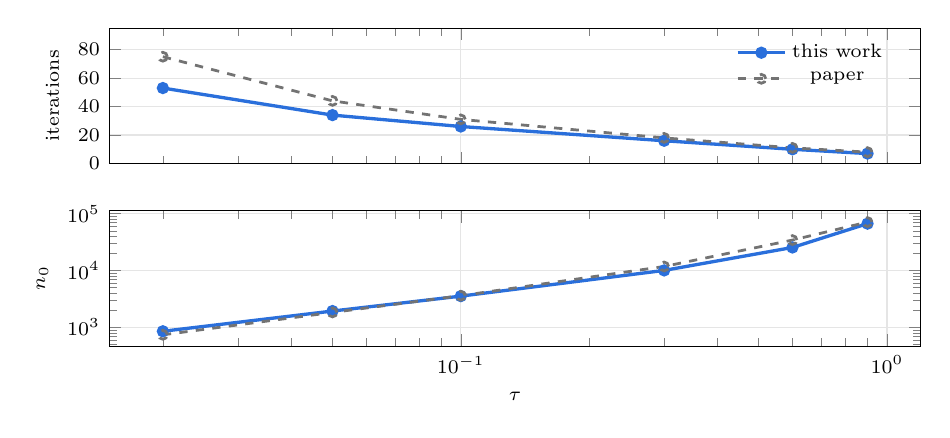
\begin{tikzpicture}
      \begin{groupplot}[group style={group size=1 by 2,vertical sep=6mm,xticklabels at=edge bottom},
          width=0.98\linewidth,height=3.3cm,xmode=log,xmin=0.015,xmax=1.2,
          tick label style={font=\scriptsize},label style={font=\scriptsize},
          legend style={font=\scriptsize,draw=none,fill=none},grid=major,grid style={black!10}]
        \nextgroupplot[ylabel={iterations},legend pos=north east,ymin=0,ymax=95]
          \addplot[schwarz,line width=1.2pt,mark=*,mark size=1.6pt] coordinates {(0.02,53)(0.05,34)(0.1,26)(0.3,16)(0.6,10)(0.9,7)};
          \addplot[black!55,dashed,line width=1pt,mark=o,mark size=1.6pt] coordinates {(0.02,75)(0.05,44)(0.1,31)(0.3,18)(0.6,11)(0.9,8)};
          \legend{this work,paper}
        \nextgroupplot[ylabel={$n_0$},ymode=log,xlabel={$\tau$}]
          \addplot[schwarz,line width=1.2pt,mark=*,mark size=1.6pt] coordinates {(0.02,853)(0.05,1936)(0.1,3545)(0.3,10052)(0.6,25473)(0.9,66910)};
          \addplot[black!55,dashed,line width=1pt,mark=o,mark size=1.6pt] coordinates {(0.02,739)(0.05,1831)(0.1,3608)(0.3,11784)(0.6,34402)(0.9,71385)};
      \end{groupplot}
    \end{tikzpicture}
  \end{columns}
  \vspace{1mm}
  
  \small 
  Larger $\tau$: more eigenvectors per subdomain, fewer iterations; one-level ASM does not reach $10^{-8}$.
\end{frame}

\begin{frame}{8. Reproduction of the paper: strong scaling (Fig.~4) and Table 2}
  \begin{columns}[c,onlytextwidth]
    \column{0.55\textwidth}
    \centering
    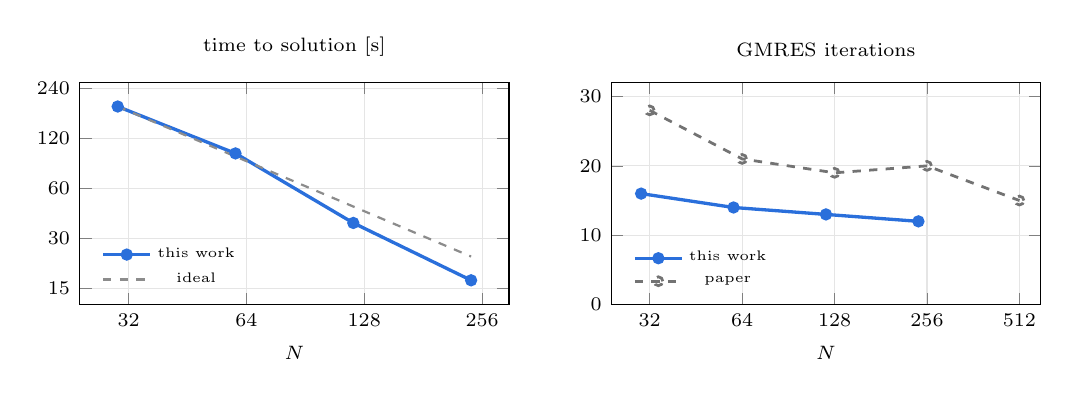
\begin{tikzpicture}
      \begin{groupplot}[group style={group size=2 by 1,horizontal sep=13mm},
          width=0.58\linewidth,height=4.4cm,xmode=log,log basis x=2,
          xtick={32,64,128,256,512},xticklabels={32,64,128,256,512},
          tick label style={font=\scriptsize},label style={font=\scriptsize},title style={font=\scriptsize},
          legend style={font=\tiny,draw=none,fill=none},grid=major,grid style={black!10},xlabel={$N$}]
        \nextgroupplot[ymode=log,title={time to solution [s]},xmin=24,xmax=300,ymin=12,ymax=260,
                       ytick={15,30,60,120,240},log ticks with fixed point,legend pos=south west]
          \addplot[schwarz,line width=1.2pt,mark=*,mark size=1.6pt] coordinates {(30,186.8)(60,97.5)(120,37.2)(240,16.8)};
          \addplot[black!45,dashed,line width=0.8pt] coordinates {(30,186.8)(240,23.35)};
          \legend{this work,ideal}
        \nextgroupplot[title={GMRES iterations},ymin=0,ymax=32,xmin=24,xmax=600,legend pos=south west]
          \addplot[schwarz,line width=1.2pt,mark=*,mark size=1.6pt] coordinates {(30,16)(60,14)(120,13)(240,12)};
          \addplot[black!55,dashed,line width=1pt,mark=o,mark size=1.6pt] coordinates {(32,28)(64,21)(128,19)(256,20)(512,15)};
          \legend{this work,paper}
      \end{groupplot}
    \end{tikzpicture}\\
    {\scriptsize\muted{3D (4.1), $\nu=10^{-2}$, $8\cdot10^6$ unknowns, $\tau=0.3$, \texttt{nev}$=60$.}}
    \column{0.42\textwidth}
    \small
    \begin{itemize}
      \item Iterations \alert{bounded in $N$}, as in the paper.
      \item Superlinear speed-up ($11.1\times$ for $8\times$ the processes): setup is 96--97\% of the
            time, and LU of $A_{ii}$ and eigensolves grow faster than linearly with $n_i$.
      \item Table 2 (convection--diffusion): same trends; $n_0$ smaller than the paper
            ($0.5$--$0.6\times$ in 2D, $\approx0.2\times$ in 3D): FV stencils couple the overlap to fewer
            outside nodes $\Rightarrow$ less lumping.
    \end{itemize}
  \end{columns}
\end{frame}

% =============================================================================================
\section{Bubble flow: extras}
% =============================================================================================

\begin{frame}{9. Bubble flow: the problem}
  \begin{columns}[c,onlytextwidth]
    \column{0.60\textwidth}
    \small\setlength{\parskip}{7pt}%
    \textbf{\color{schwarz}Pressure equation} of an incompressible two-phase flow:
    \begin{gather*}
      -\nabla\cdot(\beta\nabla p)=f,\qquad \beta=\frac{1}{\rho},\\
      \rho=\alpha\rho_g+(1-\alpha)\rho_l,\qquad \frac{\rho_l}{\rho_g}=10^3\ \text{(air in water)}.
    \end{gather*}
    
    Discretized with cell-centred finite volumes $\implies A$ is SPD, diagonally dominant and an M-matrix.

    \textbf{\color{schwarz}Test case} of the next slides: $128\times128$ cells, five bubbles of radius
    $0.07$, $p=0$ on the top side (\code{matgen bubbles2d}, same matrix as in the report).
    \column{0.36\textwidth}
    \centering
    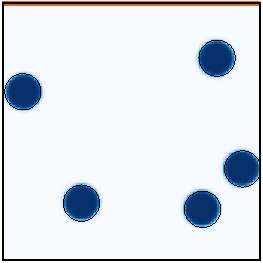
\includegraphics[width=0.92\linewidth]{fig/bubble_alpha.pdf}\\[1.5mm]
    {\scriptsize gas fraction $\alpha$ \quad \textcolor{gamg}{\rule[0.5ex]{4mm}{1.2pt}}\ $p=0$}
  \end{columns}
\end{frame}

\begin{frame}{9. Bubble flow: why it is hard}
  \begin{columns}[c,onlytextwidth]
    \column{0.57\textwidth}
    \small\setlength{\parskip}{7pt}%
    \textbf{\color{schwarz}Near-kernel modes.} In the gas $\beta$ is $10^3$ times larger. A pressure field
    flat inside a bubble, varying only in the liquid, has an energy $\int\beta|\nabla p|^2$ about $10^3$
    times smaller than the same shape with its gradient in the gas: every bubble away from the Dirichlet
    boundary adds one such mode.

    \textbf{\color{schwarz}Hard for multigrid:} the modes are not smooth, flat in the bubble and bent at the
    interface. GAMG agglomerates by face area, blind to $\beta$, and leaves them to the smoother.

    \vspace{2mm} 
    Good application of the preconditioner: the local eigenproblems use only $A$ and find these
    modes, whatever the bubble shape.

    \column{0.39\textwidth}
    \centering
    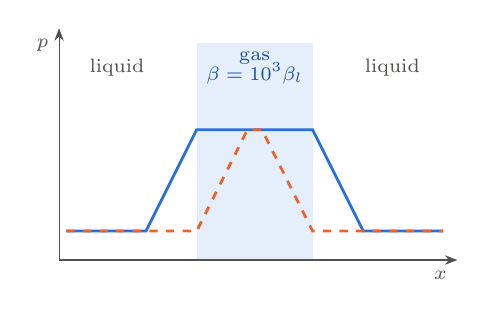
\begin{tikzpicture}[x=0.92mm,y=0.92mm]
      \fill[schwarz!12] (19,0) rectangle (35,30);
      \node[font=\scriptsize,schwarz!70!black,align=center] at (27,26.5) {gas\\[-1pt]$\beta=10^3\beta_l$};
      \node[font=\scriptsize,ink2] at (8,26.5) {liquid};
      \node[font=\scriptsize,ink2] at (46,26.5) {liquid};
      \draw[ink2,-{Stealth[length=1.6mm]}] (0,0) -- (55,0) node[below left=0.5pt,font=\scriptsize] {$x$};
      \draw[ink2,-{Stealth[length=1.6mm]}] (0,0) -- (0,32) node[below left=0.5pt,font=\scriptsize] {$p$};
      % low-energy mode: flat in the gas, gradient in the liquid
      \draw[schwarz,line width=1pt] (1,4) -- (12,4) -- (19,18) -- (35,18) -- (42,4) -- (53,4);
      % same shape, gradient in the gas
      \draw[gamg,line width=1pt,dashed] (1,4) -- (19,4) -- (26,18) -- (28,18) -- (35,4) -- (53,4);
    \end{tikzpicture}\\[1mm]
    {\scriptsize
    \textcolor{schwarz}{\rule[0.5ex]{5mm}{1pt}}\ $\nabla p$ in the liquid: low energy\\
    \textcolor{gamg}{\rule[0.5ex]{1.6mm}{1pt}\,\rule[0.5ex]{1.6mm}{1pt}}\ $\nabla p$ in the gas: $\approx10^3\times$ the energy\\[1mm]
    \muted{1D cut through a bubble}}
  \end{columns}
\end{frame}

\begin{frame}{9. Bubble flow: near-kernel modes}
  \begin{columns}[c,onlytextwidth]
    \column{0.70\textwidth}
    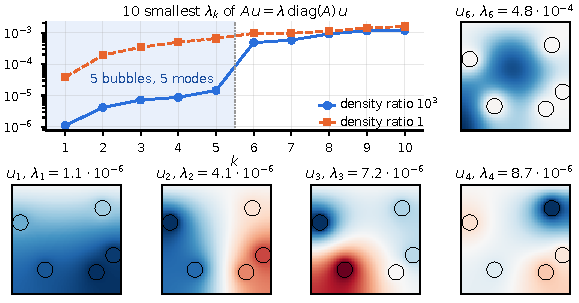
\includegraphics[width=\linewidth]{fig/bubble_modes.pdf}
    \column{0.27\textwidth}
    \small\setlength{\parskip}{7pt}%
    \textbf{\color{schwarz}Spectrum.} Five eigenvalues lie $33$--$430\times$ below $\lambda_6$, one per
    bubble. With uniform density the gap disappears.

    \textbf{\color{schwarz}Eigenvectors.} $u_1,\dots,u_5$ are flat on every bubble and bend only in the
    liquid. $u_6$, above the gap, vanishes in the gas.
  \end{columns}
  \vspace{5mm}
  \noindent\begin{minipage}{\textwidth}\tiny\muted{Eigenpairs of $Au=\lambda\,\mathrm{diag}(A)\,u$
  computed with SciPy (\code{scripts/bubble\_modes.py}).}\end{minipage}
\end{frame}

\begin{frame}{9. Bubble flow: the PISO time loop}
  \cmfocus{runTimeLoop}
  %\mapbadge\Wextra
  \begin{columns}[c,onlytextwidth]
    \column{0.57\textwidth}
    \small\setlength{\parskip}{5pt}%
    \textbf{\color{schwarz}PISO} couples pressure and velocity in transient incompressible
    solvers. Every time step
    transports the interface, predicts the velocity and then corrects it two or three times.

    \textbf{\color{schwarz}Each corrector} solves the pressure equation and makes the fluxes
    divergence-free. Its coefficient, $1/a_P$ of the momentum equation ($\approx\Delta t/\rho$), is frozen
    during the step: \alert{same matrix}, new right-hand side.

    \textbf{\color{schwarz}From one step to the next} the bubbles move: same sparsity pattern, new values
    near the interfaces.

    \textbf{\color{schwarz}In the tests} \code{matgen} moves the bubbles by half a cell per step; three
    correctors, each from $x_0=0$ with a random $b$.
    \column{0.41\textwidth}
    \centering
    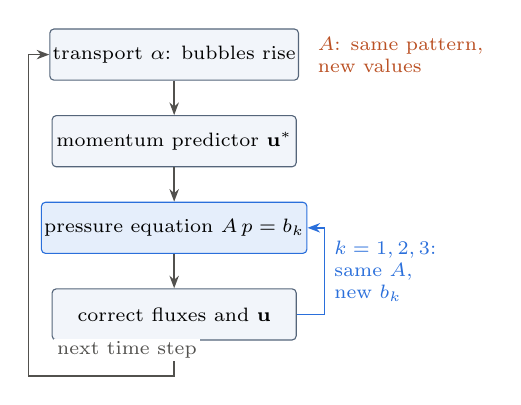
\begin{tikzpicture}[x=1mm,y=1mm,
        st/.style={draw=boxedge,fill=boxfill,rounded corners=1.5pt,minimum width=31mm,minimum height=6.5mm,
                   font=\scriptsize,align=center,inner sep=1pt},
        ar/.style={-{Stealth[length=1.6mm]},line width=0.6pt,draw=ink2}]
      \node[st] (al) at (0,0)   {transport $\alpha$: bubbles rise};
      \node[st] (mo) at (0,-11) {momentum predictor $\mathbf u^*$};
      \node[st,fill=schwarz!12,draw=schwarz] (pe) at (0,-22) {pressure equation $A\,p=b_k$};
      \node[st] (co) at (0,-33) {correct fluxes and $\mathbf u$};
      \draw[ar] (al) -- (mo);
      \draw[ar] (mo) -- (pe);
      \draw[ar] (pe) -- (co);
      \draw[ar,schwarz] (co.east) -- ++(3.5,0) |- node[pos=0.25,right,font=\scriptsize,align=left]{$k=1,2,3$:\\same $A$,\\new $b_k$} (pe.east);
      \draw[ar] (co.south) -- ++(0,-4.5) -| ++(-18.5,0) |- (al.west);
      \node[font=\scriptsize,ink2,fill=white,inner sep=1pt] at (-6,-37.5) {next time step};
      \node[font=\scriptsize,gamg!80!black,align=left,anchor=west] at (17,0) {$A$: same pattern,\\new values};
    \end{tikzpicture}
  \end{columns}
\end{frame}

\begin{frame}{9. Bubble flow: what can be kept}
  \cmfocus{runTimeLoop,ReusePolicy,Preconditioner}
  %\mapbadge\Wextra
  \small
  \textbf{\color{schwarz}Three update levels.} Before every solve \code{Preconditioner::update(UpdateLevel)}
  receives one of three levels, and the setup is split by \alert{what each part depends on}:
  \begin{center}
  \footnotesize
  \begin{tabular}{@{}llccc@{}}
    \toprule
    Depends on & Data & \code{Reuse} & \code{Refactorize} & \code{Rebuild}\\
    \midrule
    graph of $A$ & overlap, halo, patterns, $D_i$ & kept & kept & kept\\
    pattern of $A_{ii}$ & symbolic factorization & kept & kept & redone\\
    values of $A$ & $A_{ii}$, $A(\Omega_I,\Omega_i)$, $s_i$; numerical LU of $A_{ii}$ & kept & redone & redone\\
    values of $A$ and $V$ & $A_{00}$ and its factorization & kept & redone & redone\\
    values of $A$ & $\At_{ii}$, eigenproblems, $V_i$ & kept & \textbf{old basis} & redone\\
    \bottomrule
  \end{tabular}
  \end{center}

  \vspace{2mm}
  \begin{columns}[T,onlytextwidth]
    \column{0.48\textwidth}
    \footnotesize
    \textbf{\color{schwarz}Correctors 2 and 3} find the same values: \code{Subdomain::updateValues()}
    detects it with one reduction and the level becomes \code{Reuse}. New values cost one halo exchange
    and an indexed copy.
    \column{0.48\textwidth}
    \footnotesize
    \textbf{\color{schwarz}One decision for all ranks:} \code{agree()} takes the highest level over the
    ranks. The measured times differ slightly from rank to rank, and a rank rebuilding alone would
    deadlock in the collectives of the coarse level.
  \end{columns}
\end{frame}

\begin{frame}{9. Bubble flow: when to rebuild (P1)}
  \cmfocus{ReusePolicy,runTimeLoop}
  %\mapbadge\Wextra
  \begin{columns}[c,onlytextwidth]
    \column{0.52\textwidth}
    \small\setlength{\parskip}{6pt}%
    \textbf{\color{schwarz}Aging.} A refactorization keeps $A_{ii}$ and $A_{00}$ exact, but the basis $V_i$
    was computed for bubbles that have moved: the iterations grow.

    \textbf{\color{schwarz}Waste.} With $d$ decades of residual reduction in $k$ iterations, $q=k/d$, and
    $q_{\mathrm{ref}}$ its value right after a rebuild, every solve wastes
    $(k-q_{\mathrm{ref}}\,d)\,t_{\mathrm{it}}$ seconds because of the old basis.

    \textbf{\color{schwarz}Break-even.} \code{ReusePolicy} rebuilds when the waste since the last rebuild
    reaches the extra cost of a rebuild over a refactorization, both \alert{measured} in the run (lower
    medians). This rent-or-buy rule never spends more than twice the best choice in hindsight, with no
    threshold to tune.
    \column{0.45\textwidth}
    \centering\footnotesize
    \begin{tabular}{@{}lrrr@{}}
      \toprule
      Problem & \code{off} & \code{auto} & gain\\
      \midrule
      bubbles $128^3$ & 3.47\,s & 0.611\,s & \good{5.7$\times$}\\
      bubbles $192^3$ & 16.0\,s & 2.62\,s & \good{6.1$\times$}\\
      conv.-diff.\ $100^3$ & 1.25\,s & 0.169\,s & \good{7.4$\times$}\\
      \bottomrule
    \end{tabular}\\[1.5mm]
    \begin{minipage}{\linewidth}\scriptsize\muted{Cost per solve, setup included, 240 processes; bubbles with $\rho_l/\rho_g=10^3$,
    convection--diffusion non-symmetric.
    \code{off}: new setup before every solve; \code{auto}: refactorize at every step, rebuild at
    break-even.}\end{minipage}\par\vspace{3mm}
    \noindent\mapsec\Wextra{0.97\linewidth}
  \end{columns}
\end{frame}

\begin{frame}{9. Bubble flow: setup reuse on G100 (P1)}
  \cmfocus{ReusePolicy,runTimeLoop}
  %\mapbadge\Wextra
  \centering
  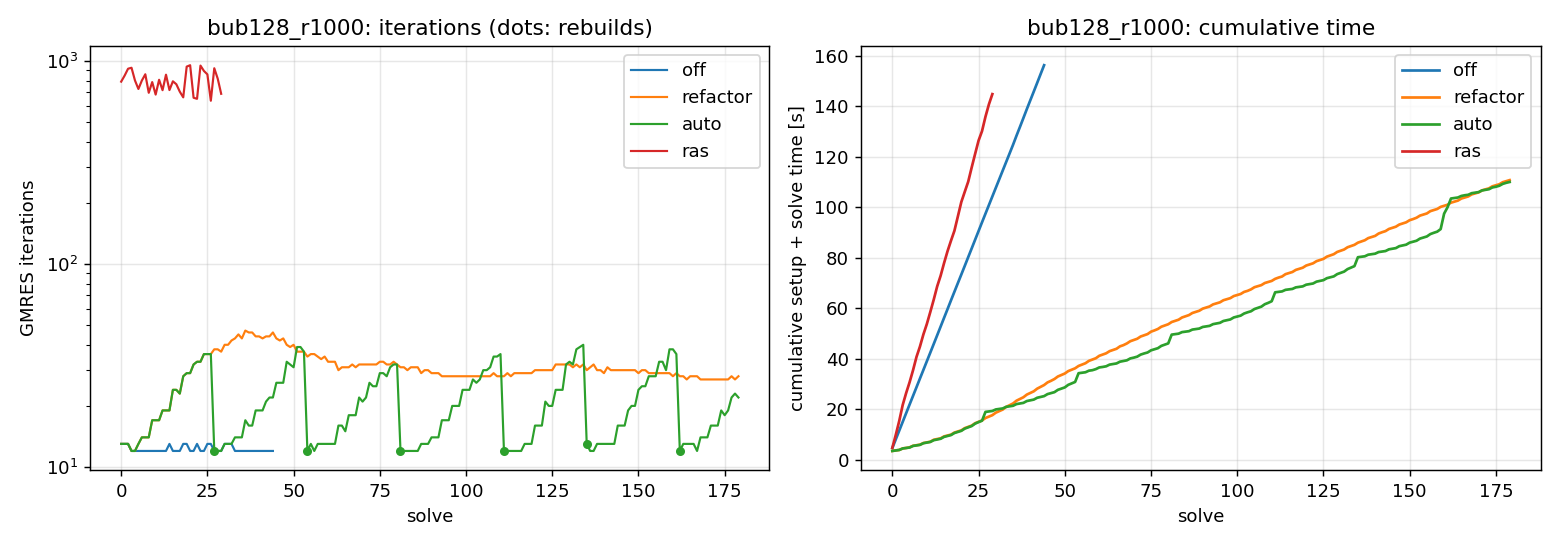
\includegraphics[width=0.92\textwidth]{fig/reuse_bub128.png}\par
  \vspace{1mm}
  \begin{columns}[T,onlytextwidth]
    \column{0.49\textwidth}
    \footnotesize
    \textbf{\color{schwarz}Iterations.} One-level RAS needs about 800. With \code{refactor} (basis never
    rebuilt) they grow from 12 to 47, then settle around 30; \code{auto} rebuilds every $\sim$9 steps,
    a saw-tooth from 12 to 31--39.
    \column{0.49\textwidth}
    \footnotesize
    \textbf{\color{schwarz}Cost.} Both reuse modes are about $6\times$ cheaper than \code{off}. Here
    \code{auto} and \code{refactor} end together (0.611 and 0.615\,s per solve): the rule does not need
    to know in advance whether rebuilding pays.
  \end{columns}
  \vfill
  \noindent\begin{minipage}{\textwidth}\tiny\muted{Bubbles $128^3$, $\rho_l/\rho_g=10^3$, 240 processes, GMRES(30) to
  $10^{-8}$, 3 correctors per step; dots: rebuilds chosen by \code{auto}. The jump near solve 160 is a
  timing burst, not a rebuild.}\end{minipage}
\end{frame}

\begin{frame}{9. Bubble flow: cheaper solves (P2, P5, P7)}
  \small
  \textbf{\color{schwarz}Method.} Each phase starts from a measured bottleneck, changes one thing, passes
  the unit tests and is measured in a campaign on G100 (\code{test/*/RESULTS.md}).
  \begin{center}
  \footnotesize\setlength{\tabcolsep}{5pt}
  \begin{tabular}{@{}llll@{}}
    \toprule
    Phase & Change & \multicolumn{2}{l}{Cost per solve}\\
    \midrule
    P2 & Cholesky instead of LU for $A_{ii}$, $\widetilde A_{ii}+\sigma I$ and $A_{00}$ & \good{$-10\%$ to $-18\%$} & same iterations\\
    \addlinespace[2pt]
    P5 & at most \texttt{nev}$\,=8$ coarse vectors per subdomain & \good{$-52\%$ to $-80\%$} & rebuilds 4--6$\times$ cheaper\\
    \addlinespace[2pt]
    P7 & one AMG V-cycle instead of exact factors of $A_{ii}$ & \good{$-26\%$ to $-56\%$} & same iterations after a rebuild\\
    \bottomrule
  \end{tabular}
  \end{center}
  \vspace{1mm}
  \begin{columns}[T,onlytextwidth]
    \column{0.48\textwidth}
    \footnotesize
    \textbf{\color{schwarz}Why P7 is allowed.} Schwarz theory admits any local solver
    \alert{spectrally equivalent} to $A_{ii}^{-1}$. One V-cycle of smoothed aggregation from $x=0$ is a
    fixed linear operator, so plain GMRES stays valid. It reads about $1.5\,\mathrm{nnz}(A_{ii})$ a few
    times, while a 3D Cholesky factor has 20--35$\times$ the nonzeros of $A_{ii}$.
    \column{0.48\textwidth}
    \footnotesize
    \textbf{\color{schwarz}Measured and dropped:} incomplete Cholesky ($2.4$--$8.7\times$ the
    iterations: not spectrally equivalent), other AMG smoothers, reusing the AMG hierarchy across
    refactorizations, single-precision factors as a default, warm-started eigenvectors.
  \end{columns}
\end{frame}

% =============================================================================================
\section{Performance vs GAMG}
% =============================================================================================

\begin{frame}{10. Performance vs GAMG: setting}
  \begin{columns}[c,onlytextwidth]
    \column{0.50\textwidth}
    \small\setlength{\parskip}{6pt}%
    \textbf{\color{schwarz}Same problem on both sides.} The OpenFOAM-10 solver \code{bubblyPressureFoam}
    assembles the same equation with the \alert{same} header-only \code{BubbleField}: the matrices agree to
    $3.6\cdot10^{-15}$ (relative), checked in every job.

    \textbf{\color{schwarz}GAMG} runs with the OpenFOAM defaults, \code{faceAreaPair} agglomeration and DIC
    smoother, the fastest variant tested.

    \textbf{\color{schwarz}Schwarz} runs with $\tau=0.3$, \texttt{nev}$\,=8$, AMG local solves and reuse
    \texttt{auto}.

    \textbf{\color{schwarz}Meshes} of $192^3$, $256^3$ and $320^3$ cells (7.1--32.8\,M) on 240, 336 and 432
    processes. The cost of a solve includes setup, updates and iterations.
    \column{0.47\textwidth}
    \centering
    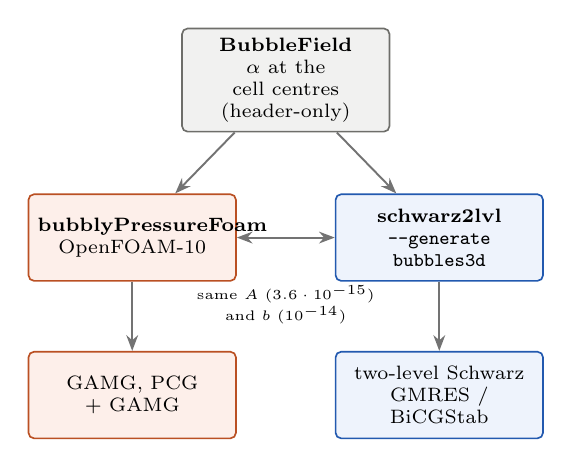
\begin{tikzpicture}[x=1mm,y=1mm,
        bx/.style={rounded corners=2pt,text width=24mm,minimum height=11mm,align=center,font=\scriptsize,line width=0.6pt},
        ar/.style={-{Stealth[length=2mm]},line width=0.7pt,draw=black!55}]
      \node[bx,draw=cmutils!80!black,fill=cmutils!12] (bf) at (19.5,26) {\textbf{BubbleField}\\ $\alpha$ at the cell centres\\ (header-only)};
      \node[bx,draw=gamg!80!black,fill=gamg!10] (of) at (0,6) {\textbf{bubblyPressureFoam}\\ OpenFOAM-10};
      \node[bx,draw=schwarz!80!black,fill=schwarz!8] (s2) at (39,6) {\textbf{schwarz2lvl}\\ \code{-{}-generate bubbles3d}};
      \draw[ar] (bf) -- (of); \draw[ar] (bf) -- (s2);
      \node[bx,draw=gamg!80!black,fill=gamg!10] (g) at (0,-14) {GAMG, PCG + GAMG};
      \node[bx,draw=schwarz!80!black,fill=schwarz!8] (t) at (39,-14) {two-level Schwarz\\ GMRES / BiCGStab};
      \draw[ar] (of) -- (g); \draw[ar] (s2) -- (t);
      \draw[{Stealth[length=2mm]}-{Stealth[length=2mm]},line width=0.7pt,draw=black!55] (of.east) -- (s2.west);
      \node[font=\tiny,align=center,fill=white,inner sep=1pt] at (19.5,-2.5) {same $A$ ($3.6\cdot10^{-15}$)\\ and $b$ ($10^{-14}$)};
    \end{tikzpicture}
  \end{columns}
\end{frame}

\begin{frame}{10. Performance vs GAMG: every solve from zero}
  \begin{columns}[c,onlytextwidth]
    \column{0.53\textwidth}
    \footnotesize
    Cost per solve [s], Schwarz / GAMG, \code{relTol} $10^{-2}$ of the OpenFOAM residual, 16 steps
    $\times$ 3 correctors:\par\vspace{1.5mm}
    \centering
    \begin{tabular}{@{}lccc@{}}
      \toprule
      & 240 proc. & 336 proc. & 432 proc.\\
      \midrule
      $192^3$ & 0.316 / 0.567 & 0.258 / 0.570 & 0.206 / 0.563\\
              & \good{1.79$\times$} & \good{2.21$\times$} & \good{2.73$\times$}\\[2pt]
      $256^3$ & 0.986 / 1.99 & 0.724 / 1.65 & 0.573 / 1.48\\
              & \good{2.02$\times$} & \good{2.28$\times$} & \good{2.59$\times$}\\[2pt]
      $320^3$ & 2.38 / 4.74 & 1.80 / 3.39 & 1.12 / 2.74\\
              & \good{1.99$\times$} & \good{1.88$\times$} & \good{2.44$\times$}\\
      \bottomrule
    \end{tabular}\par\vspace{1mm}
    \raggedright{\scriptsize\muted{Schwarz with GMRES(30); GAMG with DIC. Ratio GAMG / Schwarz, $>1$: Schwarz
    faster.}\par}
    \column{0.43\textwidth}
    \small\setlength{\parskip}{6pt}%
    \textbf{\color{schwarz}Always faster:} the gain holds on all \alert{9 configurations}, $1.8$--$2.7\times$.

    \textbf{\color{schwarz}At a tight tolerance}, $\|r\|_2/\|b\|_2\le10^{-8}$ on 240 processes, it grows to
    \good{$2.0\times$} at $192^3$ and \good{$4.3\times$} at $256^3$: GAMG goes from 139 to 271 V-cycles,
    Schwarz needs 51 iterations at both sizes.

    \textbf{\color{schwarz}Setup and updates} are about $30\%$ of the Schwarz cost at $10^{-2}$.
  \end{columns}
\end{frame}

\begin{frame}{10. Performance vs GAMG: strong scaling}
  \centering
  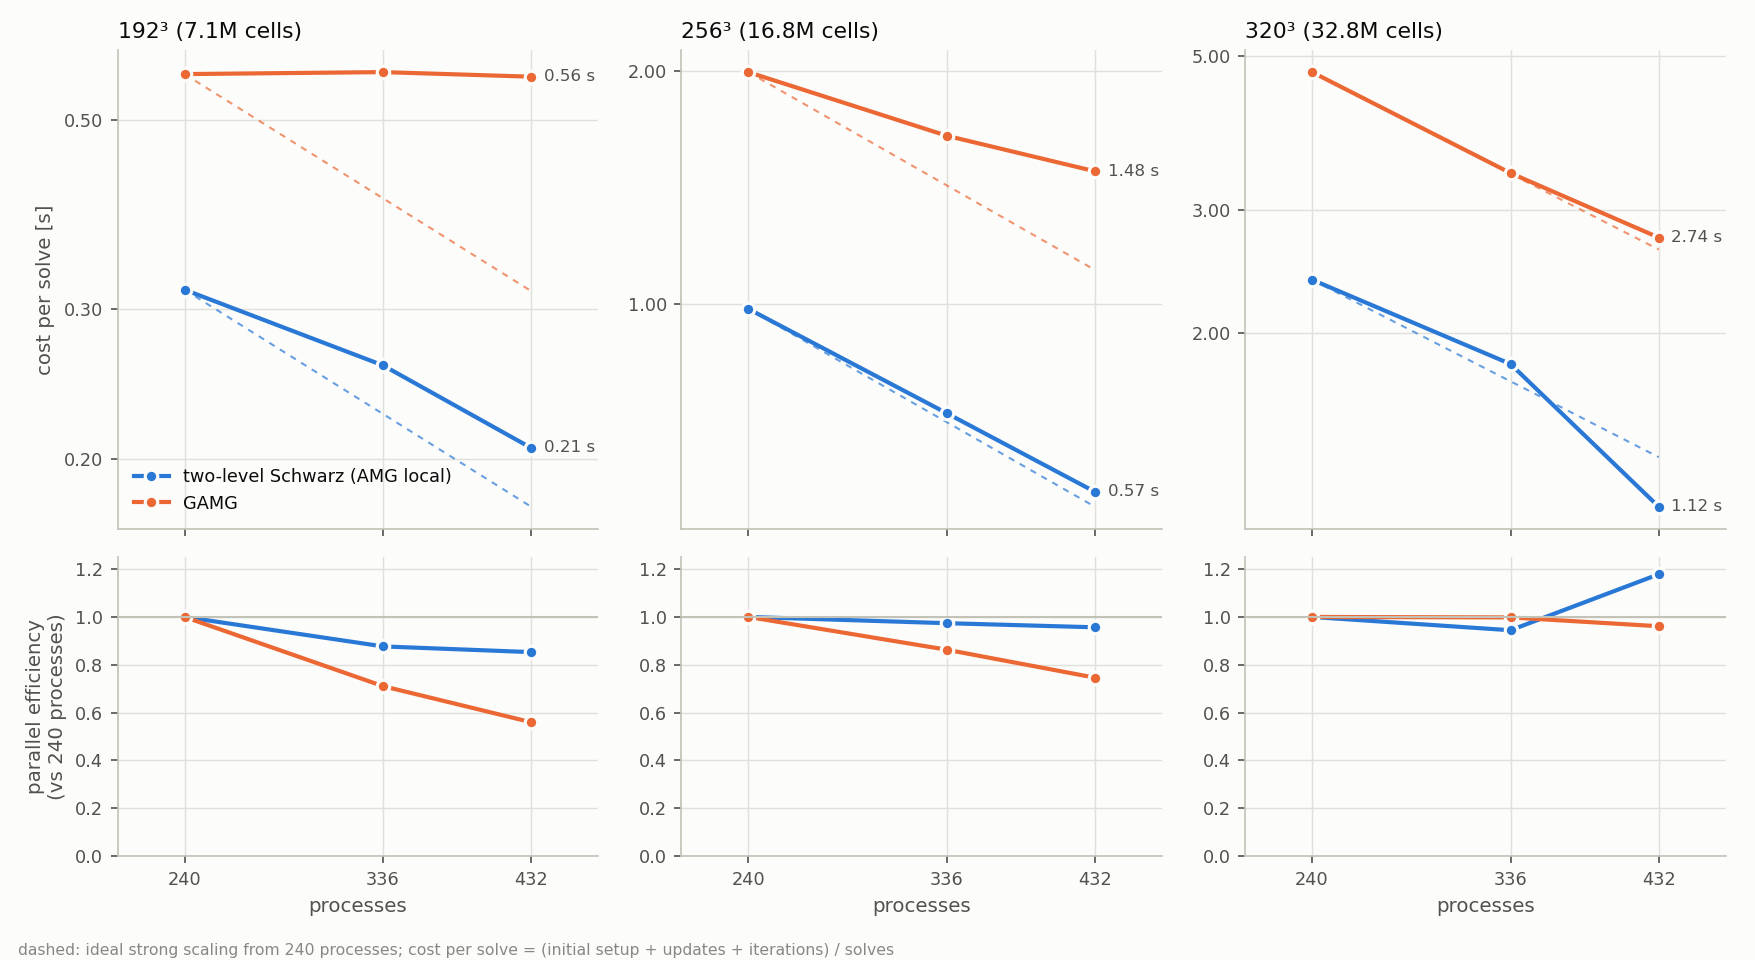
\includegraphics[height=0.70\textheight]{fig/gamg_strong.png}\par\vspace{1.5mm}
  \small\textbf{\color{schwarz}Parallel efficiency} from 240 to 432 processes: Schwarz \good{0.85 / 0.96 / 1.18},
  GAMG 0.56 / 0.75 / 0.96 ($192^3$ / $256^3$ / $320^3$).
\end{frame}

\begin{frame}{10. Performance vs GAMG: where the gain comes from}
  \centering
  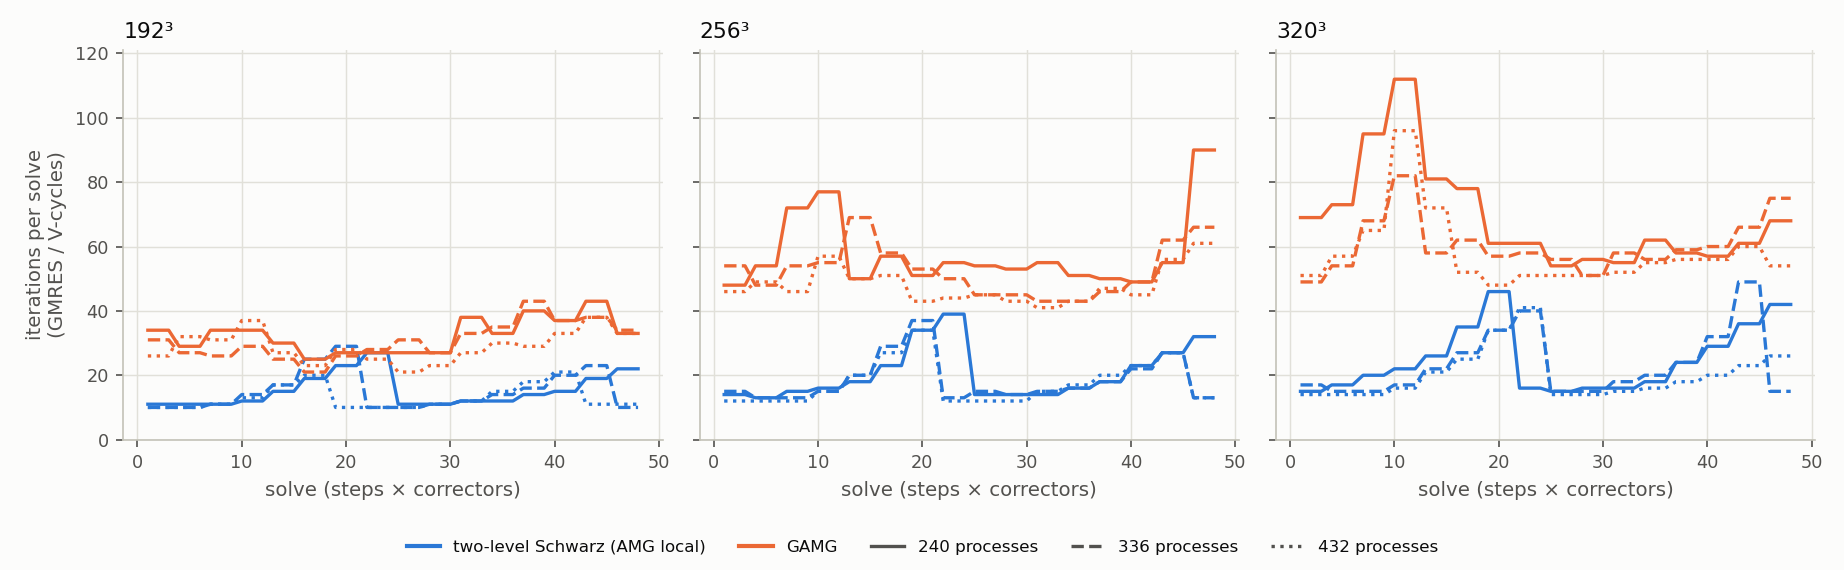
\includegraphics[width=0.96\textwidth]{fig/gamg_iterations.png}\par\vspace{2mm}
  \begin{columns}[c,onlytextwidth]
    \column{0.48\textwidth}
    \small
    \textbf{\color{schwarz}Same cost per iteration.} One Schwarz iteration costs about one GAMG V-cycle:
    $34.8$ vs $34.5$\,ms at $256^3$, $68.9$ vs $68.8$\,ms at $320^3$. The gain is \alert{entirely in the
    iterations}, $2.0$--$2.9\times$ fewer.
    \column{0.48\textwidth}
    \small
    \textbf{\color{schwarz}Iterations.} From $192^3$ to $320^3$ GAMG goes from 32 to 69 V-cycles, Schwarz
    after a rebuild from 11 to 15. The saw-tooth is the coarse space that \alert{ages} as the bubbles move,
    until the break-even rebuild.
  \end{columns}
\end{frame}

\begin{frame}{10. Performance vs GAMG: Krylov method}
  \centering
  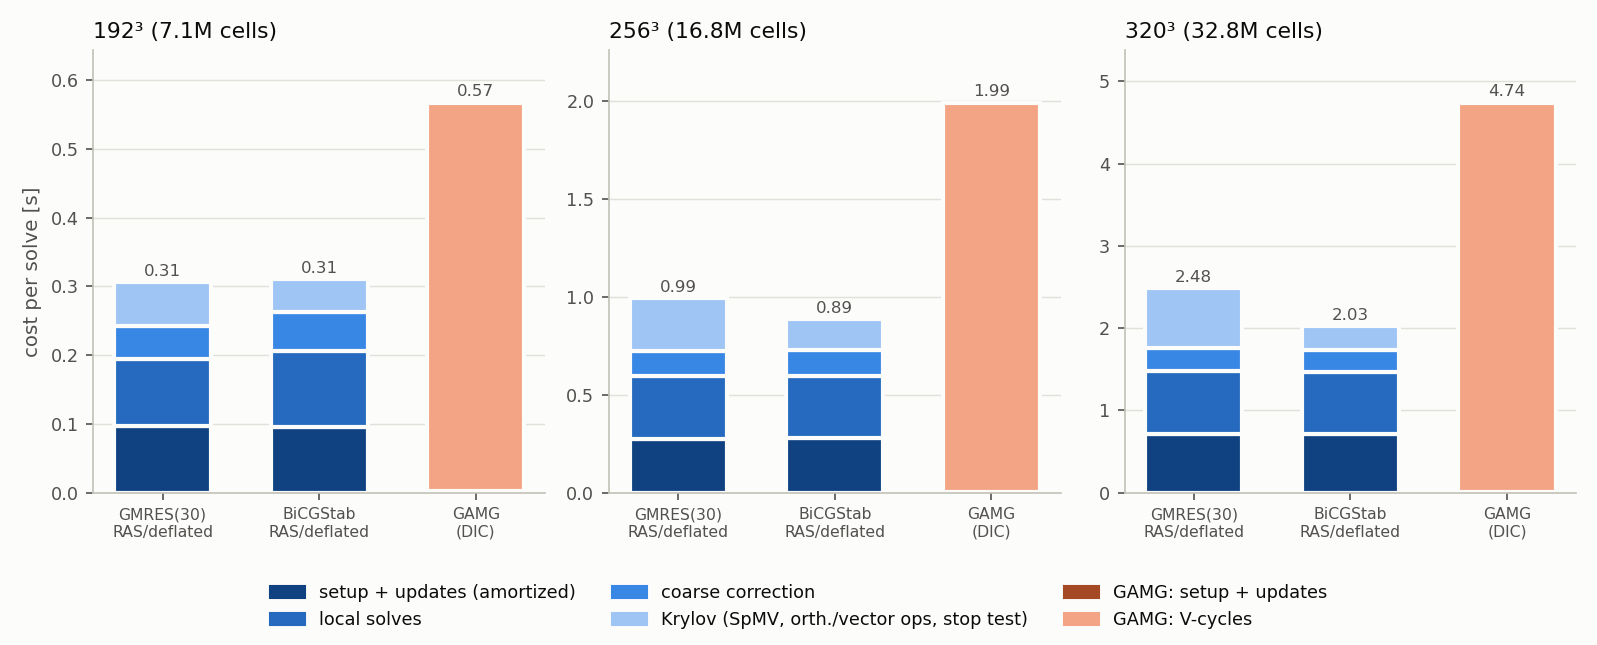
\includegraphics[width=0.76\textwidth]{fig/gamg_krylov.png}\par\vspace{2mm}
  \begin{columns}[T,onlytextwidth]
    \column{0.48\textwidth}
    \small
    \textbf{\color{schwarz}GMRES} pays CGS2 and the OpenFOAM stopping test with $O(j)$ passes over the basis,
    and $j$ grows with the mesh.
    \column{0.48\textwidth}
    \small
    \textbf{\color{schwarz}BiCGStab} needs $1.04$--$1.20\times$ the applications, each $0.72$--$0.85\times$ as
    expensive: \good{$0.89$} and \good{$0.82\times$} the cost of GMRES at $256^3$ and $320^3$ ($1.02\times$ at
    $192^3$). It is OpenFOAM's \code{PBiCGStab}, the natural host of a port.
  \end{columns}
\end{frame}

\begin{frame}{10. Performance vs GAMG: a PIMPLE-like time loop}
  \begin{columns}[T,onlytextwidth]
    \column{0.47\textwidth}
    \small\setlength{\parskip}{5pt}%
    \textbf{\color{schwarz}Closer to an OpenFOAM run.} The right-hand side is the $p_{rgh}$ source of
    \code{interFoam}, on the interfaces and with zero sum over every bubble. Every solve starts from the
    previous solution (\alert{warm start}); the correctors stop at \code{relTol} 0.05, the last one at
    \code{tolerance} $10^{-7}$.

    \begin{exampleblock}{Decision rule, fixed before the run}
      \footnotesize Port only if $\ge1.5\times$ faster than the best OpenFOAM variant at both process counts.
    \end{exampleblock}
    \column{0.50\textwidth}
    \centering\footnotesize
    \begin{tabular}{@{}rrrrr@{}}
      \toprule
      Mesh & Proc. & Schwarz & GAMG & ratio\\
      \midrule
      $192^3$ & 240 & 0.605 & 0.581 & 0.96$\times$\\
      $256^3$ & 240 & 1.68  & 1.97  & 1.17$\times$\\
      $320^3$ & 240 & 4.30  & 5.08  & 1.18$\times$\\
      $192^3$ & 432 & 0.358 & 0.647 & \good{1.81$\times$}\\
      $256^3$ & 432 & 0.911 & 1.51  & \good{1.66$\times$}\\
      $320^3$ & 432 & 2.06  & 2.79  & 1.35$\times$\\
      \bottomrule
    \end{tabular}\par\vspace{0.5mm}
    {\scriptsize\muted{Cost per time step [s]: 3 correctors, setup and rebuilds included, 24 steps.}\par}
  \end{columns}
  \vspace{3mm}
  \small\textbf{\color{schwarz}Outcome.} Faster than GAMG in 5 of 6 configurations, but the $1.5\times$
  threshold is reached only at 432 processes on the two smaller meshes: a port is \alert{not justified as it
  stands}.
\end{frame}

\begin{frame}{10. Performance vs GAMG: reading the PIMPLE-like result}
  \centering
  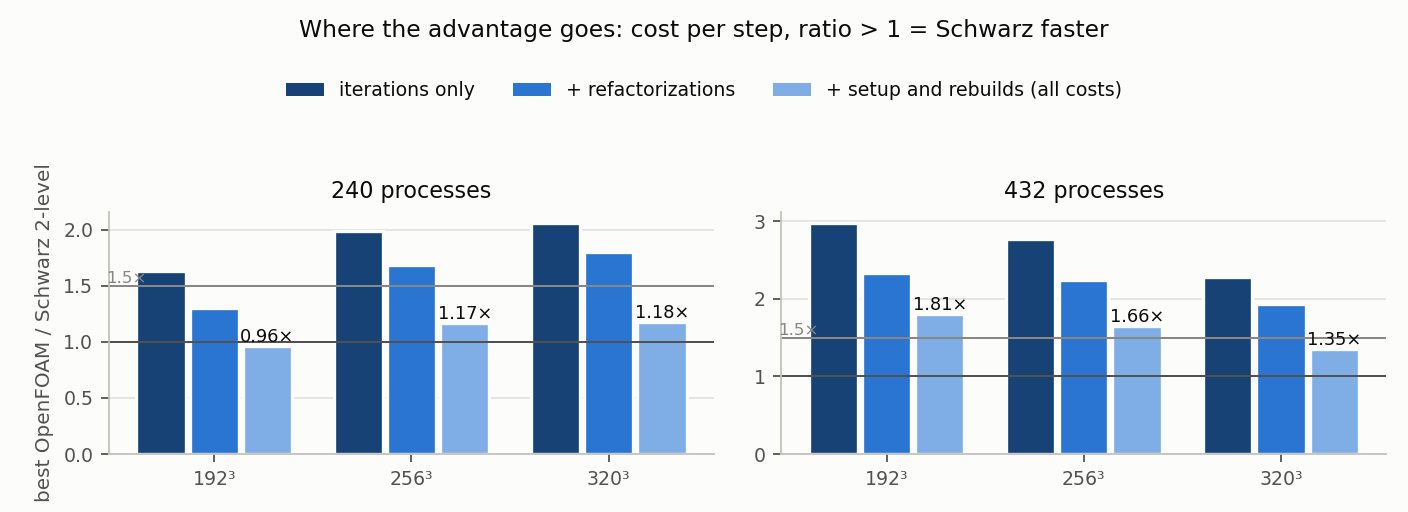
\includegraphics[width=0.80\textwidth]{fig/gamg_warm_ratio.png}\par\vspace{2mm}
  \begin{columns}[T,onlytextwidth]
    \column{0.48\textwidth}
    \small
    \textbf{\color{schwarz}The gain moves to the last corrector}, $2.0$--$4.1\times$. On the first two, 1.3
    decades from a good guess, GAMG is $1.2$--$1.7\times$ cheaper: little of the error lies in the bubble
    modes.
    \column{0.48\textwidth}
    \small
    \textbf{\color{schwarz}Setup and rebuilds} take \alert{39--43\%} of the Schwarz cost. The iterations became
    cheap, the setup did not.
  \end{columns}
\end{frame}

\begin{frame}{10. Performance vs GAMG: why the gap narrows in the time loop}
  \begin{columns}[c,onlytextwidth]
    \column{0.50\textwidth}
    \small\setlength{\parskip}{6pt}%
    \textbf{\color{schwarz}GAMG} cannot reduce the error along the bubble modes $u_k$, flat on
    each bubble and invisible to a coarsening blind to $\beta$.

    \textbf{\color{schwarz}The error} depends on $b$ and $x_0$. From $x_0=0$:
    \[
      e_0 = x = \sum_k \frac{u_k^\top b}{\lambda_k}\,u_k ,
    \]
    the tiny $\lambda_k$ amplify the bubble modes, unless $u_k^\top b\approx0$.
    \column{0.47\textwidth}
    \centering\footnotesize\setlength{\tabcolsep}{3pt}
    \begin{tabular}{@{}lcc@{}}
      \toprule
      & from zero & time loop\\
      \midrule
      $b$ & $\alpha$ on the bubbles & $p_{rgh}$ source\\
      \addlinespace[2pt]
      $u_k^\top b$ & $\neq0$ & $\approx0$\\
      \addlinespace[2pt]
      $x_0$ & $0$ & previous $x$\\
      \addlinespace[2pt]
      energy in $u_1,\dots,u_{10}$ & \textbf{99\%} & $\boldsymbol{<0.1\%}$\\
      \addlinespace[2pt]
      GAMG / Schwarz & \good{1.8--2.7$\times$} & 0.96--1.81$\times$\\
      \bottomrule
    \end{tabular}
  \end{columns}
  \vspace{3mm}
  \small
  In the time loop the $p_{rgh}$ source sums to zero over every bubble and the warm
  start already carries the bubble levels: the test from zero was the \alert{worst case for GAMG}.
  
  \textbf{\color{schwarz}The coarse space is still needed:} one-level RAS costs $2.9$--$5.7\times$ GAMG
  (420--700 applications on the last corrector).
\end{frame}

% =============================================================================================
\section{Conclusions}
% =============================================================================================

\begin{frame}{11. Conclusions}
  \small
  \begin{columns}[T,onlytextwidth]
    \column{0.48\textwidth}
    {\textbf{\color{schwarz}Implementation}\par}\vspace{0.8mm}
    {\color{boxedge}\hrule height 0.5pt}\vspace{2mm}
    \footnotesize\setlength{\parskip}{5pt}%
    \textbf{\color{schwarz}Fully distributed} C++17/MPI library: its only input is \code{LocalSystem}, the rows
    that an OpenFOAM processor owns.

    \textbf{\color{schwarz}Run-time strategies} (local and coarse solvers, Krylov method, reuse) sit behind
    small interfaces and factories; templates only where just the types vary.

    \textbf{\color{schwarz}Section 4 of the paper} is reproduced on 240 processes, and the distributed parts
    are checked against sequential references.
    \column{0.48\textwidth}
    {\textbf{\color{gamg}Bubbly Flows}\par}\vspace{0.8mm}
    {\color{boxedge}\hrule height 0.5pt}\vspace{2mm}
    \footnotesize\setlength{\parskip}{5pt}%
    \textbf{\color{gamg}Setup reuse}, a small coarse space and AMG local solves make a solve about
    $30\times$ cheaper ($16.0\to0.51$\,s at $192^3$ on 240 processes).

    \textbf{\color{gamg}From zero} the method is $1.8$--$2.7\times$ faster than GAMG and scales better:
    the gain is algorithmic, it comes from the iterations.

    \textbf{\color{gamg}In a PIMPLE-like loop} the ratio is $0.96$--$1.81\times$ per step, and the setup is
    about $40\%$ of the cost.
  \end{columns}
  \vspace{3mm}
  \begin{block}{Next step}
    \footnotesize A coarse space that \alert{follows the bubbles} at the cost of a refactorization: keep the
    eigenvectors of the last rebuild and add indicator vectors of the gas regions of each subdomain
    ($O(n_i)$). A port would be an \code{lduMatrix::preconditioner} inside \code{PBiCGStab}, with the state
    in a \code{MeshObject}.
  \end{block}
\end{frame}

\end{document}
